\section{Background estimation}

   The irreducible background for the $\Pgg+$\met\ signal is the SM process $Z\Pgg\rightarrow\Pgn\Pagn\Pgg$. Other SM backgrounds include $\PW\Pgg$, $\PW\rightarrow \Pe\Pgn$, $\PW\rightarrow \mu\Pgn$, $\PW\rightarrow \tau\Pgn$, $\Pgg$+jet, multijet (referred to as QCD background) and diphoton events. Background events that do not come from collision processes are also considered in the analysis. These backgrounds can be divided broadly into three categories: 

\begin{itemize}
 \item Backgrounds estimated with Monte Carlo (MC) simulation: $Z\Pgg\rightarrow\Pgn\Pagn\Pgg$, $Z\Pgg\rightarrow\ell\ell\Pgg$, $\PW\Pgg$, $\Pgg$+jets, $\gamma\gamma$;
 \item Collision backgrounds estimated using data: jets misidentified as photons and electrons misidentified as photons;
 \item Non-collision backgrounds estimated using data. %: beam halo.
\end{itemize}


%%----MC simulation background
\subsection{Background estimates from MC simulation}

   %%----Zgamma & Wgamma
   The $Z\Pgg\rightarrow\Pgn\Pagn\Pgg$ is the irreducible background in this study. It is estimated from a MC sample generated with \MADGRAPH~\cite{Alwall:2011uj} and processed with \PYTHIA v6.426~\cite{Sjostrand:2006za} for showering and hadronization. To describe the topology of events in a realistic manner, up to two extra partons were included in the matrix elements during event generation. The final event yields are normalized using the next-to-leading-order (NLO) cross section calculated with the \MCFM event generator~\cite{MCFM}.  The $\PW\gamma$ MC simulation was also produced with \MADGRAPH, including up to two extra partons, and normalized using the NLO cross section calculated from \MCFM. 

  %% gamma+jet 
   The $\gamma+$jet is one of the most significant backgrounds in this analysis due to the presence of a genuine photon and the large production cross section. The events for this process are simulated using \MADGRAPH, processed through \PYTHIA and normalized using the LO cross section. The normalization of this background is then corrected using control sample in data for two different event classes: no-jet and one or more jets. The control sample in data is obtained using events collected with the prescaled single-photon trigger and with the \met requirement reversed to ensure orthogonality to the signal phase space. Correction factors ($C$) are derived by normalizing the event yield in the simulation to match the data in the control region, separately for events with zero jets ($C=1.7$) and one or more jets ($C=1.1$). These correction factors are then used to normalize the $\gamma+$jet event yield from simulation in the signal region. An uncertainty of $16\%$ is derived for these correction factors based on the difference between the corrected and uncorrected simulation and the relative fraction of zero jet ($\sim10\%$ of the events in the control region) and one or more jet events.

  %% Other MC backgronds
   The background estimate from the process $Z\Pgg\rightarrow\ell\ell\Pgg$ is obtained using \MADGRAPH, and the background estimates from the processes $\PW\rightarrow \mu\Pgn$, $\PW\rightarrow \tau\Pgn$ are obtained using \PYTHIA. These processes are found to contribute only to a small fraction of the total background prediction. 

  %% Scale Factors for MC backgrounds
   All simulated events are processed through a \GEANTfour-based simulation of the CMS detector \cite{GEANT} and the same reconstruction chain as the data. To take into account differences between data and simulation due to imperfect MC modeling, various scale factors (SF) are applied to correct the MC-based estimates. These SFs are defined as the ratio of the efficiency in data to the efficiency in simulation for a given selection. The SF for photon reconstruction and identification is estimated from $Z\rightarrow ee$ decays with $R_{9}>0.9$ using a standard ``tag-and-probe'' method ~\cite{CMS:2011aa} and are listed in Table~\ref{sf_id}. The trigger efficiency measured in Section \ref{sec:event_selection} is applied to the simulated samples.

%% Table for photon ID
\begin{table}[H]                                                                                         
\small
\center    
{ 
 \caption{Scale factors for the photon identification}                                                             
 \label{sf_id}                                                                                     
 \begin{tabular}{|c|c|c|c|}                                                                               
   \hline                                                                                                 
   Variable     &  \etg $[30 - 40] \GeV$ & \etg $[40 - 50] \GeV$ &  \etg $ > 50 \GeV$ \\                                      
   \hline                                                                                                 
   \hline                                                                                                 
Pixel Seed Veto & 0.995 $\pm$ 0.004 & 0.970 $\pm$ 0.016  & 1.012 $\pm$ 0.014 \\  
Photon ID ($0 < |\eta| < 0.8$) & 0.996 $\pm$ 0.010 & 0.996 $\pm$ 0.010 & 0.996 $\pm$ 0.010 \\          
Photon ID ($0.8 < |\eta| < 1.5$)& 0.996 $\pm$ 0.010 & 0.997 $\pm$ 0.010 & 0.997 $\pm$ 0.010 \\         
\hline                                                                                                    
\end{tabular}
}                                                                                       
\end{table}                                                                                               

%%----Collision data driven background
\subsection{Jets Identified as Photons Background}

  %--fake jets
  The contamination from jets misidentified as photons is estimated by using a data control sample, enriched in QCD multijet events, defined by \met $<$ 40 GeV. In this sample we measure the ratio of events that pass the signal photon identification and isolation criteria (numerator selection) relative to those that pass a looser photon identification and isolation criteria but also fail one of the nominal isolation requirements (denominator selection). The sample of events passing the numerator selection includes genuine photons whose contribution must be subtracted to obtain the true ratio of misidentified jets. This contribution is estimated by fitting templates of energy-weighted shower widths of genuine photons (determined from MC simulation of $\gamma+$jets events) and misidentified photons (determined from an isolation sideband in data) to the candidate distribution. The final corrected extrapolation factor, shown in Figure~\ref{fig:qcd_fr}, is then used to scale a sample of events in data which pass the denominator selection in addition to the other non-orthogonal event selections. 

%FIGURE 19
\begin{figure}[H]
\centering
{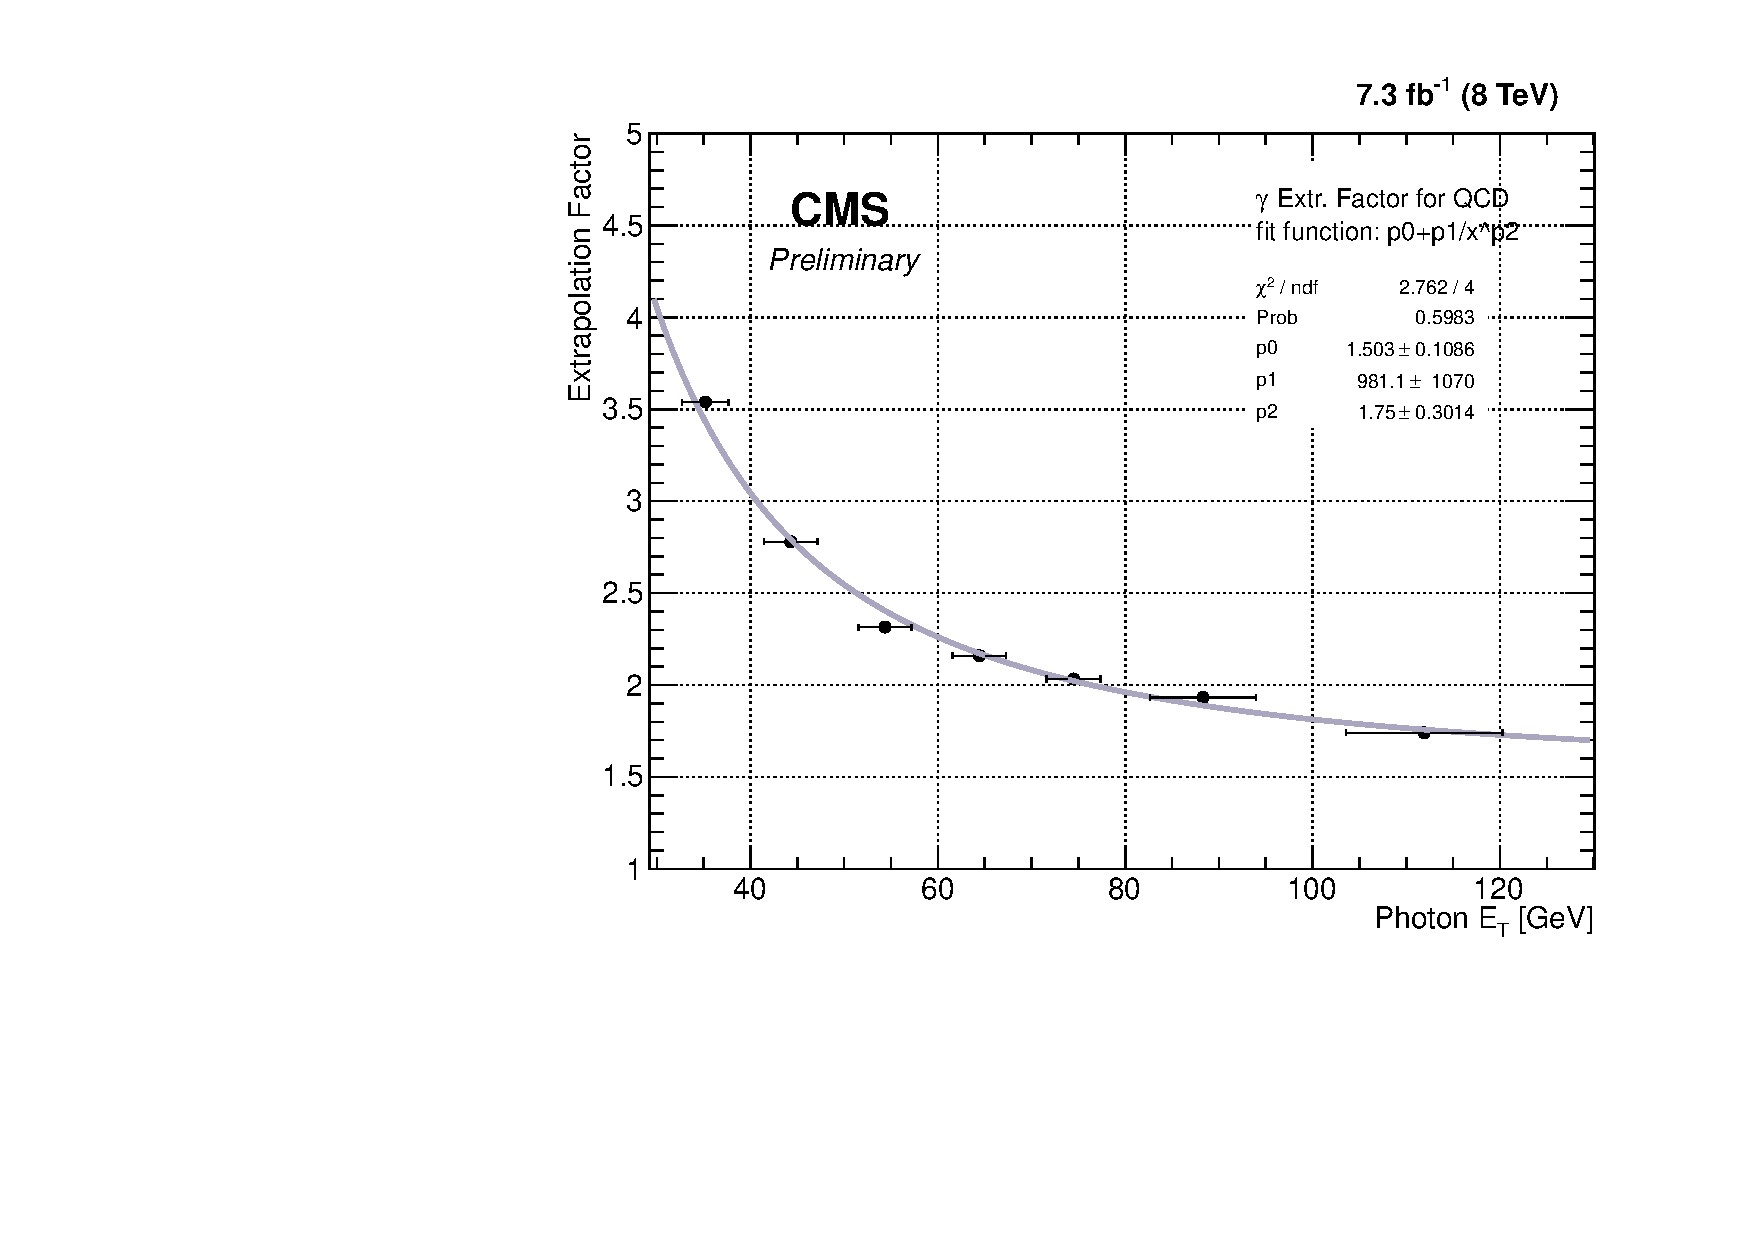
\includegraphics[scale=0.6]{figures/fitResult.pdf}}
%\newline
\caption{ Ratio of number of photons passing signal like requirement relative to those satisfying a very loose identification and isolation selection and at the same time failing at least one of the isolation criteria as a function of \etg.}
\label{fig:qcd_fr}
\end{figure}

  The systematic uncertainty in this method is dominated by the choice of the isolation sideband region and is conservatively estimated to be $35\%$ by varying the  charged-hadron isolation in the sideband region definition. The other sources of systematic uncertainty are determined by varying the bin size of the templates, the \met selection for the control region, and the loose identification requirements on the photons, and are found to be comparatively small.

\subsection{Electrons Identified as Photons Background}
\label{sec:ewk}

%%

After the cuts for QCD-like events are applied, the background that arises from electrons-faking-photons becomes the dominant for the kinematic range of this analysis. We have developed a data-driven method to obtain an accurate estimation of the electron-faking-photon background.
The main physical process behind this background is the $W\rightarrow e \nu$ production, which has a kinematic signature (fake photon \et, transverse mass, etc) very similar to the signal sample and large production cross section.

The method for estimating the electron-faking-photon contamination in the signal sample was done by constructing a control sample, similar to the signal sample, but enriched by electrons and not signal photons. This was achieved by reverting the pixel seed veto (PSV) in the photon ID requirements. The pixel seed veto cut is not the standard electron rejection tool in the $e-\gamma$ POG recommended photon ID; however, it has been shown to have a much smaller fake rate compared to the official electron rejection cut, the conversion safe electron veto. The PSV has been used in other photon-related analyses, such as the SUSY Photon and Exotica High Pt Monophoton analysis, in which the electron-faking-photon background is a dominant one.

After the control sample is created, it needs to be normalized by the number of expected electrons-faking-photons in the signal sample. This normalization can be obtained by the calculation of the fake rate of the PSV regarding electrons-faking-photons. It should be noted that this is not the fake rate of the full set of photon ID requirements, but only of the PSV cut. 

Before describing the details of this method, the following definitions must be made:

\begin{itemize}
\item $\gamma$: Objects that pass the complete $e/\gamma$ photon ID, including the PSV cut (photon object);
\item $\gamma_e$: Objects that pass the photon ID with the PSV cut reversed ($e$-fake object);
\item $N_{\gamma_e}$: Number of events in the control sample, which is made of $\gamma_e$;
\item $\epsilon_{\gamma_e}$: Efficiency of accepting $\gamma_e$ objects (including acceptance);
\item $\epsilon_{\gamma}$: Efficiency of accepting $\gamma$ objects (including acceptance);
\item $F_{e\rightarrow\gamma}$: Fake rate of the PSV cut for electrons-faking-photons.
\end{itemize}

Therefore, the number of electrons-faking-photons in the signal sample is given by
\begin{eqnarray}
N_{e \rightarrow \gamma} &=& \frac{N_{\gamma_e}}{\epsilon_{\gamma_e}} \times  F_{e\rightarrow \gamma} = N_{\gamma_e} \times R\\
R  &=& \frac{F_{e\rightarrow \gamma}}{\epsilon_{\gamma_e}}.
\end{eqnarray}

This ratio ($R$) can be related to the PSV fake rate because, for the PSV cut, the efficiency and fake rate obey the following relation:
\begin{eqnarray}
\epsilon_{\gamma_e} + F_{e\rightarrow \gamma} = 1.
\end{eqnarray}
Therefore,
\begin{eqnarray}
F_{e \rightarrow \gamma} = \frac{R}{1+R}.
\end{eqnarray}

The ratio and the fake rate can be measured using a tag-and-probe method. This method was applied to the SinglePhotonParked signal dataset. Analyzing events in which the $Z$ decays to electrons, we can reconstruct the number of events in four different cases:

\begin{itemize}
\item $Z_{e\gamma}$: one of the electrons of the $Z$ decay is identified an electron and the other is reconstructed as a photon object;
\item $Z_{e\gamma_e}$: one of the electrons of the $Z$ decay is identified as an electron and the other is reconstructed as an $e$-fake;
\item $Z_{\gamma_e\gamma}$: one of the electrons of the $Z$ decay is identified an $e$-fake and the other as a photon;
\item $Z_{\gamma_e \gamma_e}$:  both electrons of the $Z$ decay are identified as $e$-fakes;
\end{itemize} 

Therefore, we can reconstruct the number of events in each $Z$ peak case as:
\begin{eqnarray}
N_{e\gamma} &=& 2\times N^\prime\left( Z\rightarrow ee \right) \times  \epsilon_{e} \times F_{e\rightarrow\gamma}\\
N_{e\gamma_e} &=& 2\times N^\prime\left( Z\rightarrow ee \right) \times \epsilon_{e} \times \epsilon_{\gamma_e}\\
N_{\gamma \gamma_e} &=& 2\times N^\prime\left( Z\rightarrow ee \right) \times F_{e\rightarrow\gamma}\times \epsilon_{\gamma_e} \\
N_{\gamma_e \gamma_e} &=& N^\prime\left( Z\rightarrow ee \right) \times\epsilon_{\gamma_e}^2,
\end{eqnarray}
where $N_{xy}$ is the number of events of $Z$ decaying to electrons when the electrons are reconstructed as x and y, and $N^\prime\left( Z\rightarrow ee \right)$ overall number of expected $Z\rightarrow ee$ in the sample. The factors of two multiplying the first three equations are due to combinatorics.%related to the fact that there are two different objects to be identified and they can switch places.

With that system, we can infer that the calculation of the ratio can be performed in two ways:
\begin{eqnarray}
R  = \frac{F_{e\rightarrow \gamma}}{\epsilon_{\gamma_e}} = \frac{N_{e\gamma}}{N_{e\gamma_e}} = \frac{1}{2} \frac{N_{\gamma_e \gamma}}{N_{\gamma_e \gamma_e }}
\end{eqnarray}

The $Z$ shape was obtained from the template of a DY$\to ee$ MC at generator level. This template was then convoluted with a Gaussian to simulate detector resolution effects. The parameters of the Gaussian were then fitted to the obtained invariant mass distribution from the different categories detailed above. For the calculation of $N_{xy}$, the signal function was  integrated in the $\pm 2\sigma$ region to obtain the number of signal events. The fits for the $Z\rightarrow e \gamma$ and $Z \rightarrow e \gamma_e$ cases can be seen in Fig. \ref{Zep} and \ref{Zek}.
The background shape for the fit was estimated by the convolution of an error function and a decaying exponential function (RooCMSShape). The background in the Fig. \ref{Zep} is originated form the combinatorics of the electron plus non-resonant photon-like objects, such as real photons, jets faking photons and electrons faking photons originated from other interactions. Because the electron is most likely coming from the resonant Z production, the yield drops at lower values of $M_{e\gamma}$. The small disagreement between the fits and the data aroung $85$ GeV comes from the trigger and selection acceptances, since our trigger photon object selection is $30$ GeV and our probe selection \pt for this study is $35$ GeV. 

%\begin{table}[H]
%\begin{center}
%\begin{tabular}{| p{8cm} | c | c |}
%\hline
%Sample & Cross Section & Number of Events \\ \hline
%/DYToEE\_M\_20\_TuneZ2star\_8TeV \_pythia6\_v2/Summer12\_DR53X-PU\_S10 \_START53\_V7A-v1/AODSIM & 1510.0 pb & 18532820 \\ \hline
%\end{tabular}
%\caption{Sample used for gen-level template on signal fit.}
%\label{DYtoEEMC}
%\end{center}
%\end{table}

\begin{figure}[H]
\begin{center}
{\label{Zep}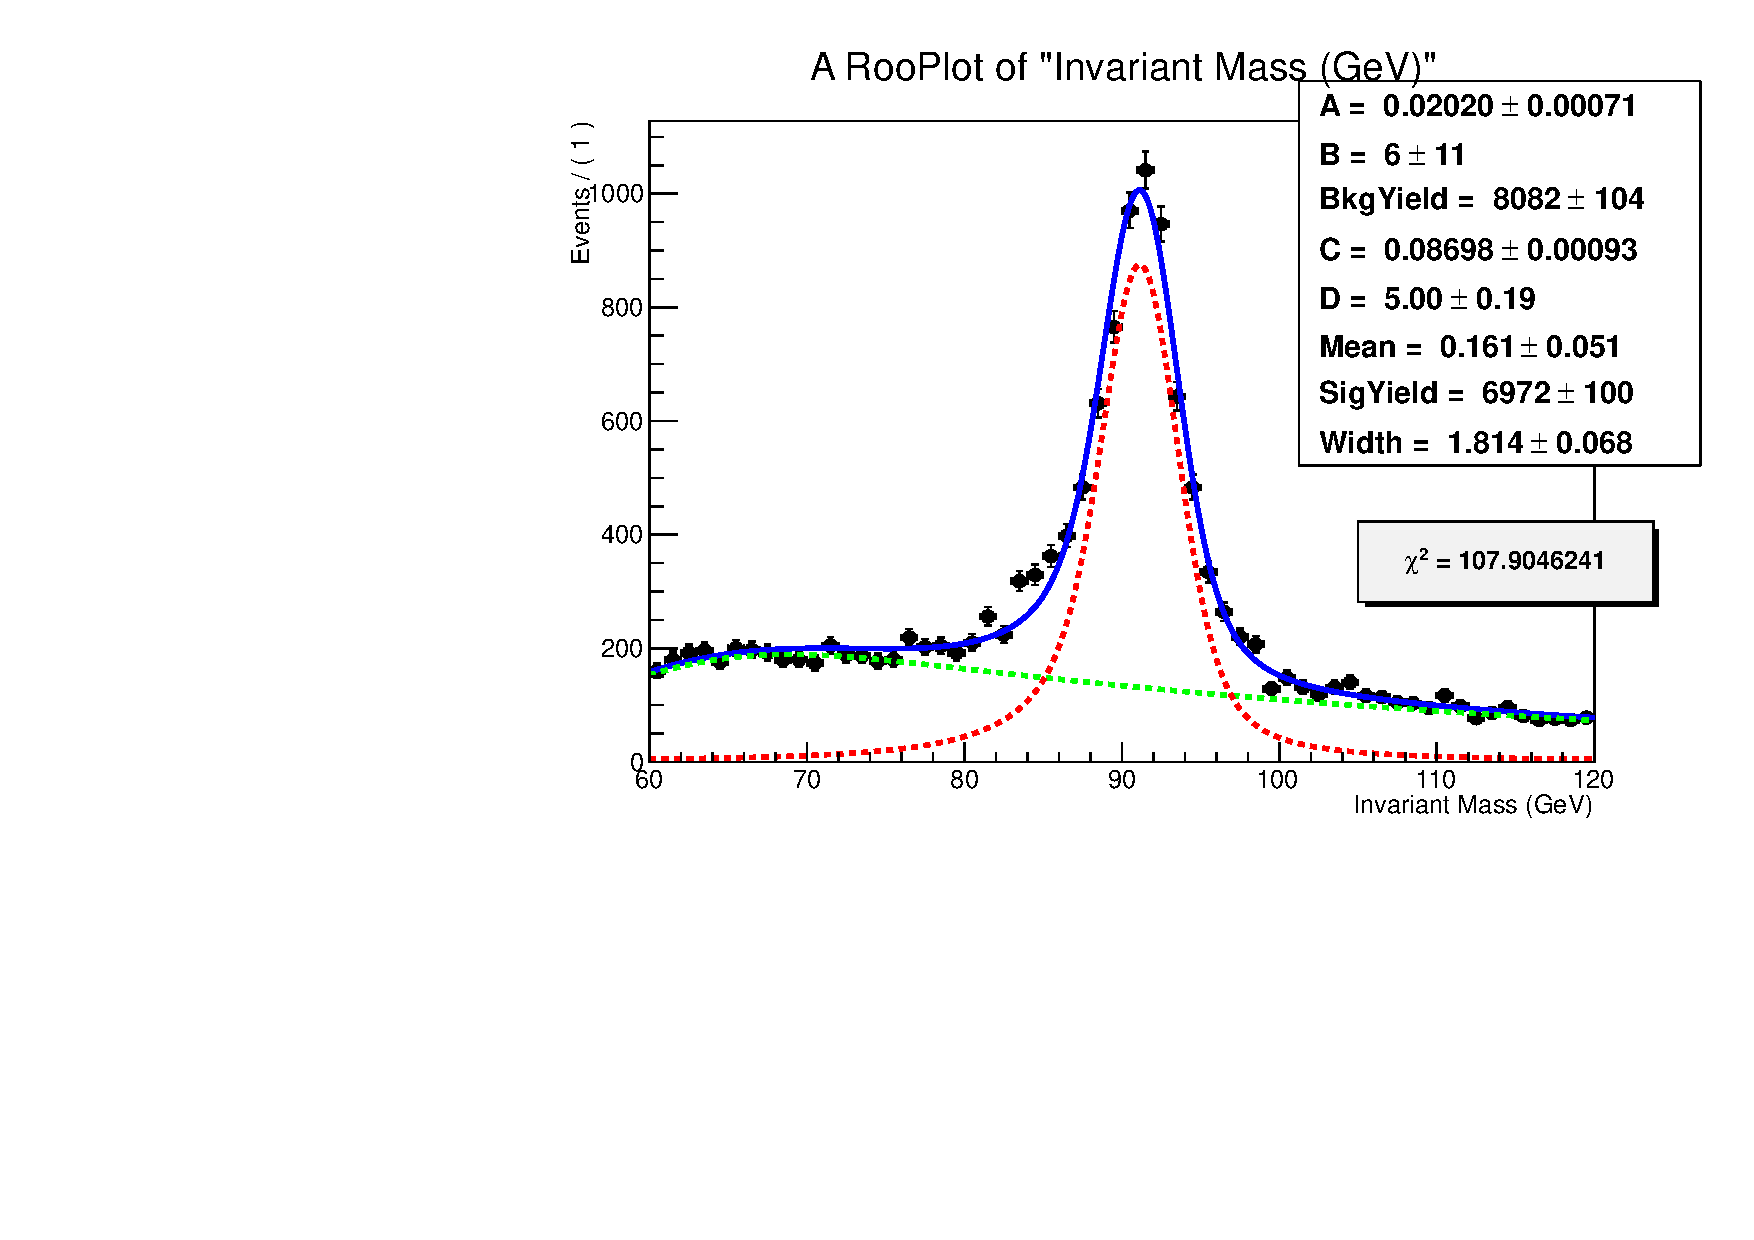
\includegraphics[width=0.45\textwidth]{efake_figs/Zep_FullMass.pdf}}
{\label{Zek}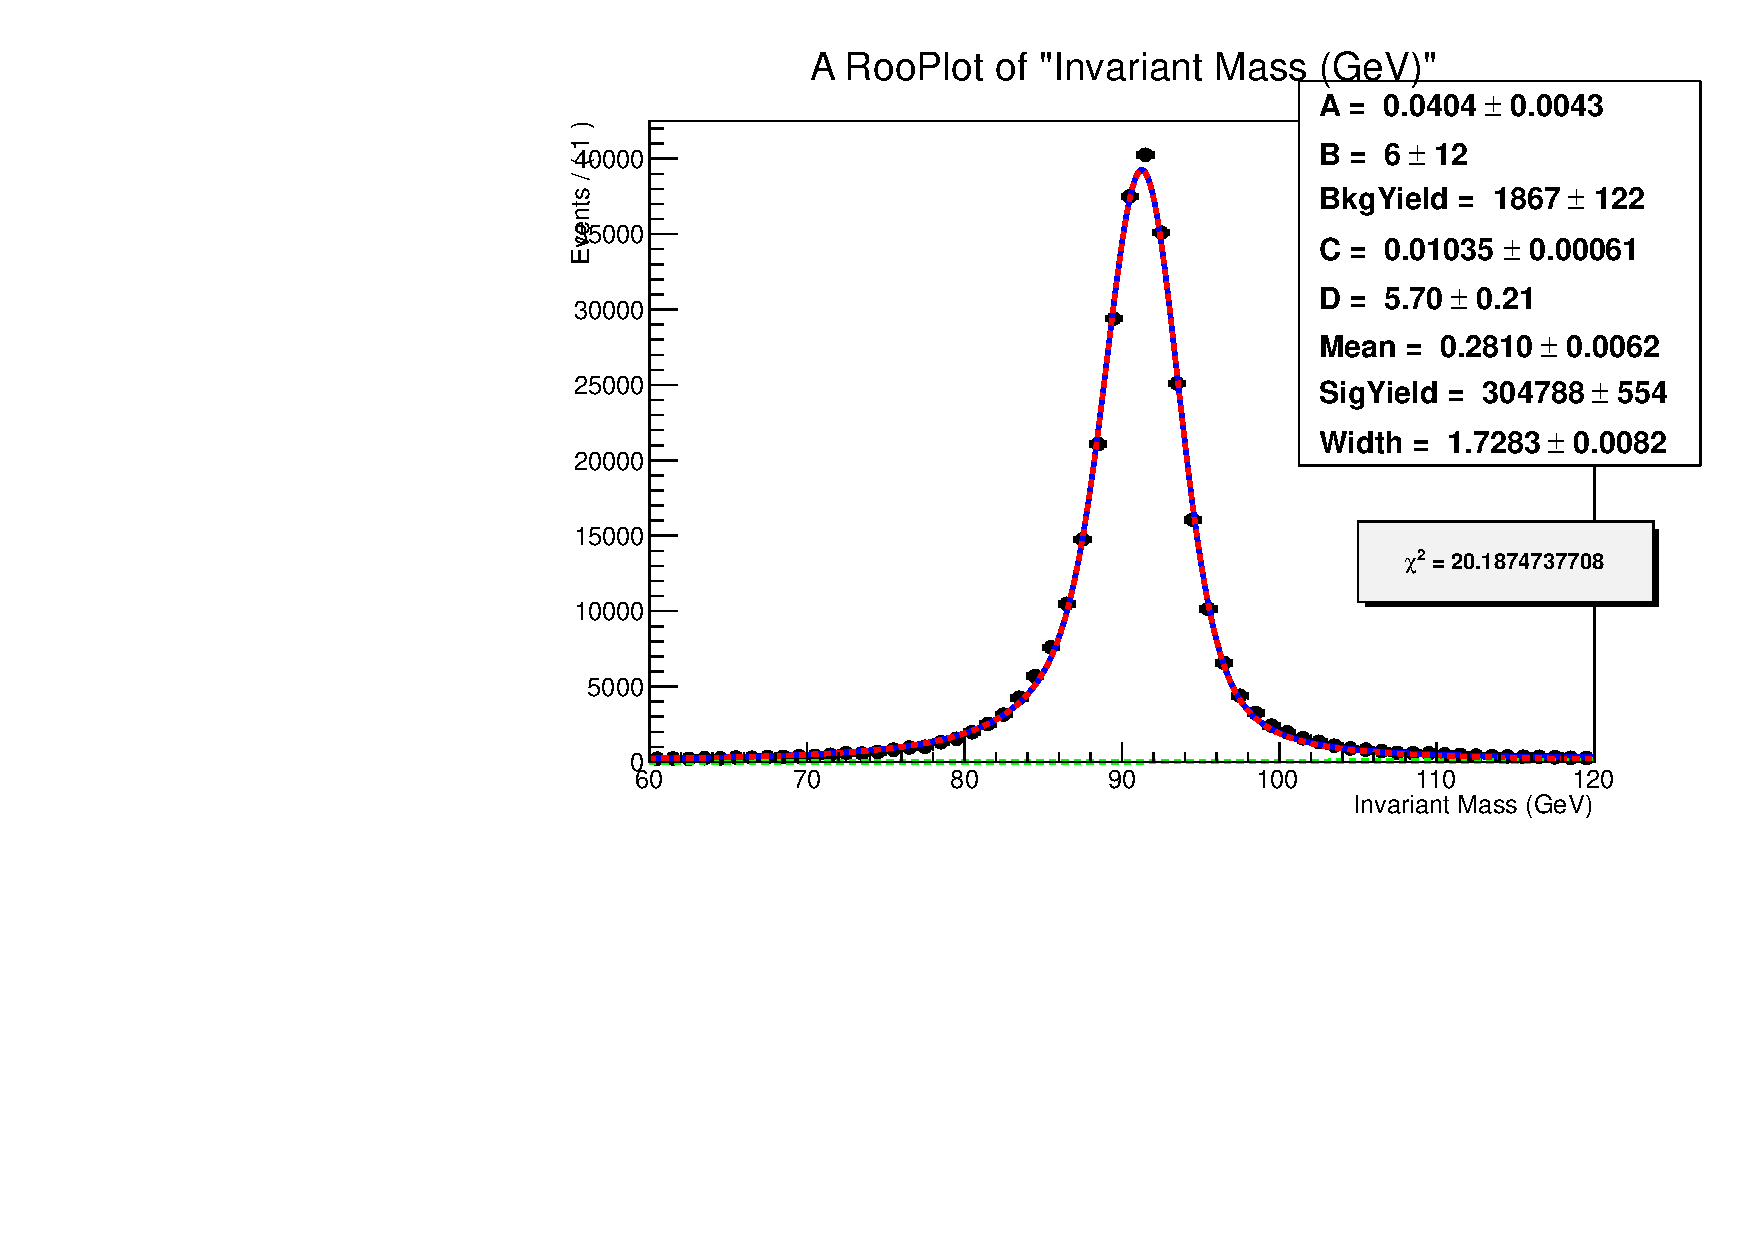
\includegraphics[width=0.45\textwidth]{efake_figs/Zek_FullMass.pdf}}
%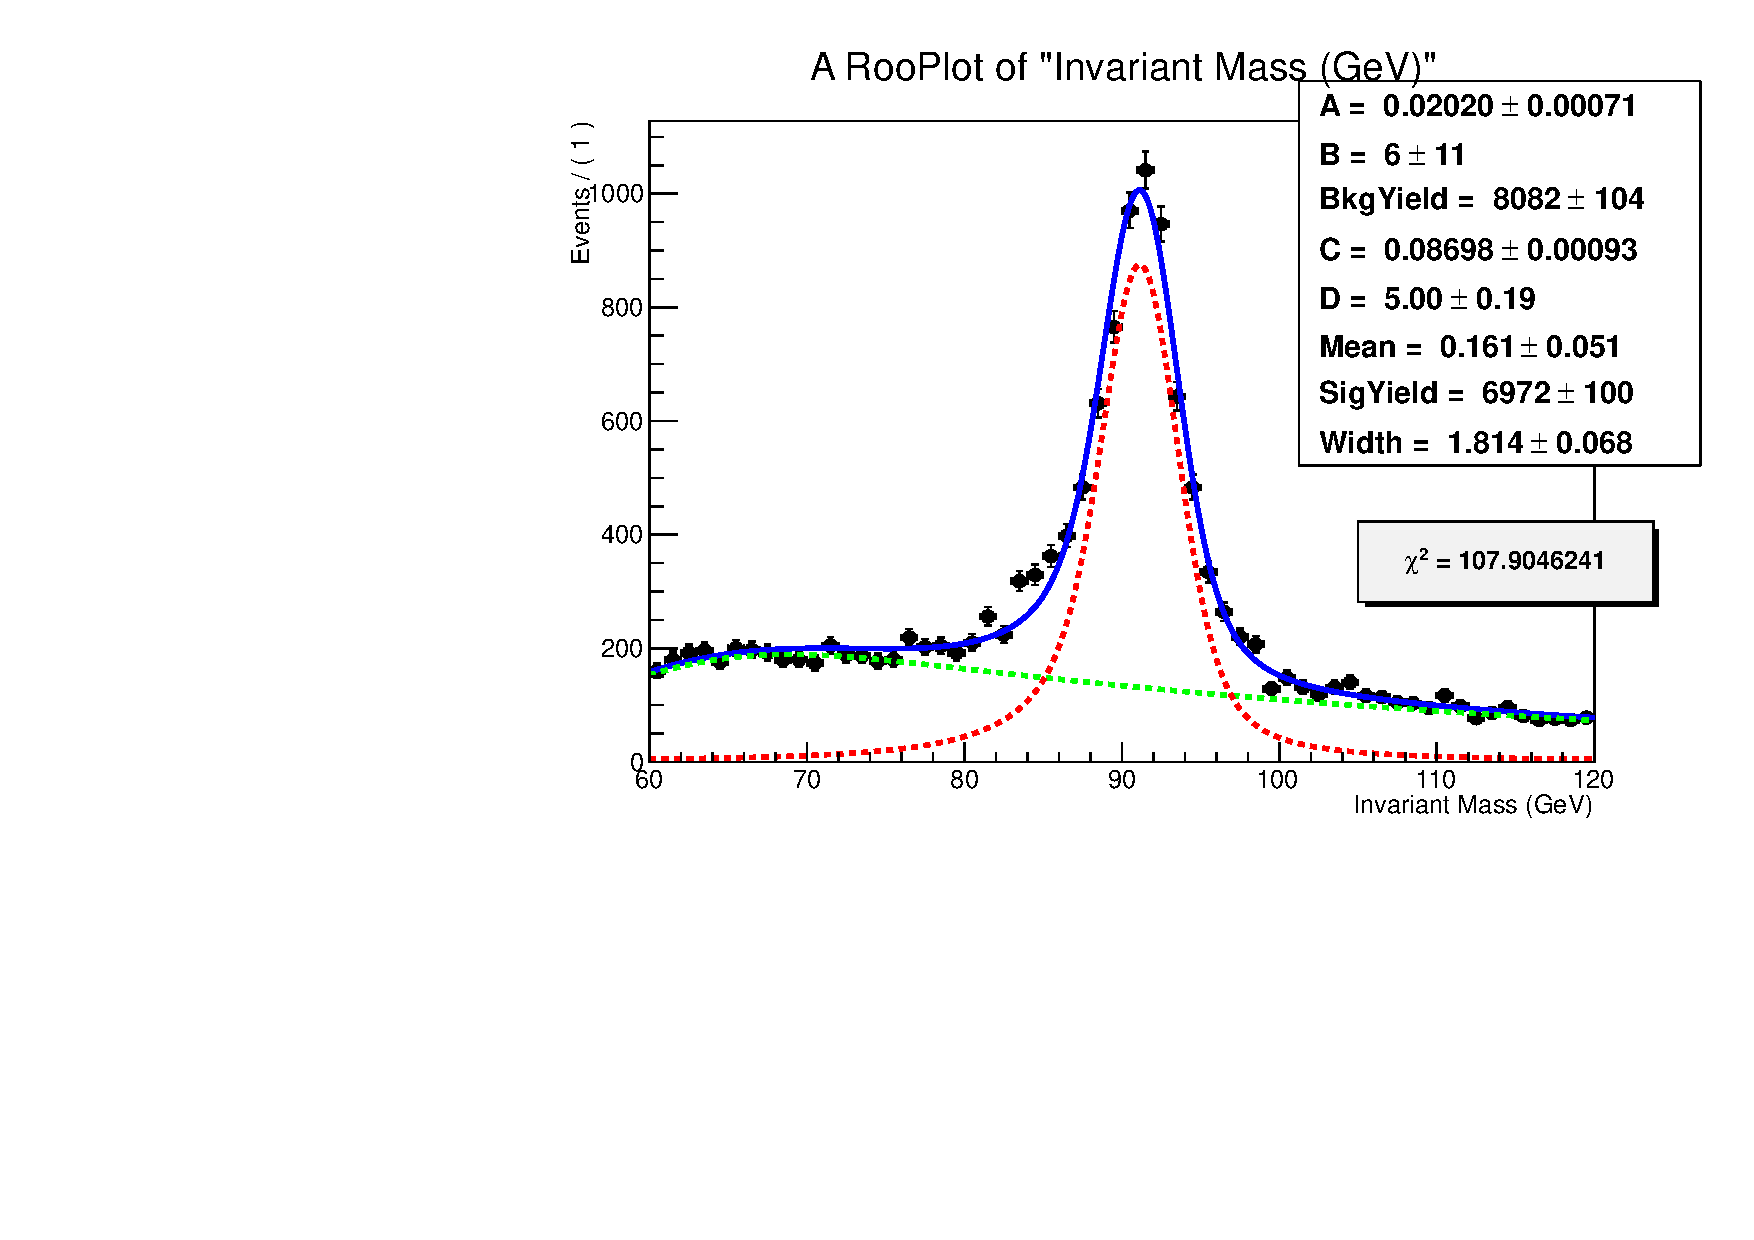
\includegraphics[scale=0.5]{efake_figs/Zep_FullMass.pdf}
\caption{Fit of the $Z$ invariant mass for the $Z\rightarrow e \gamma$ case and the $Z\rightarrow e \gamma_e$ case.}
\label{Zeall}
\end{center}
\end{figure}

%\begin{figure}[H]
%\begin{center}
%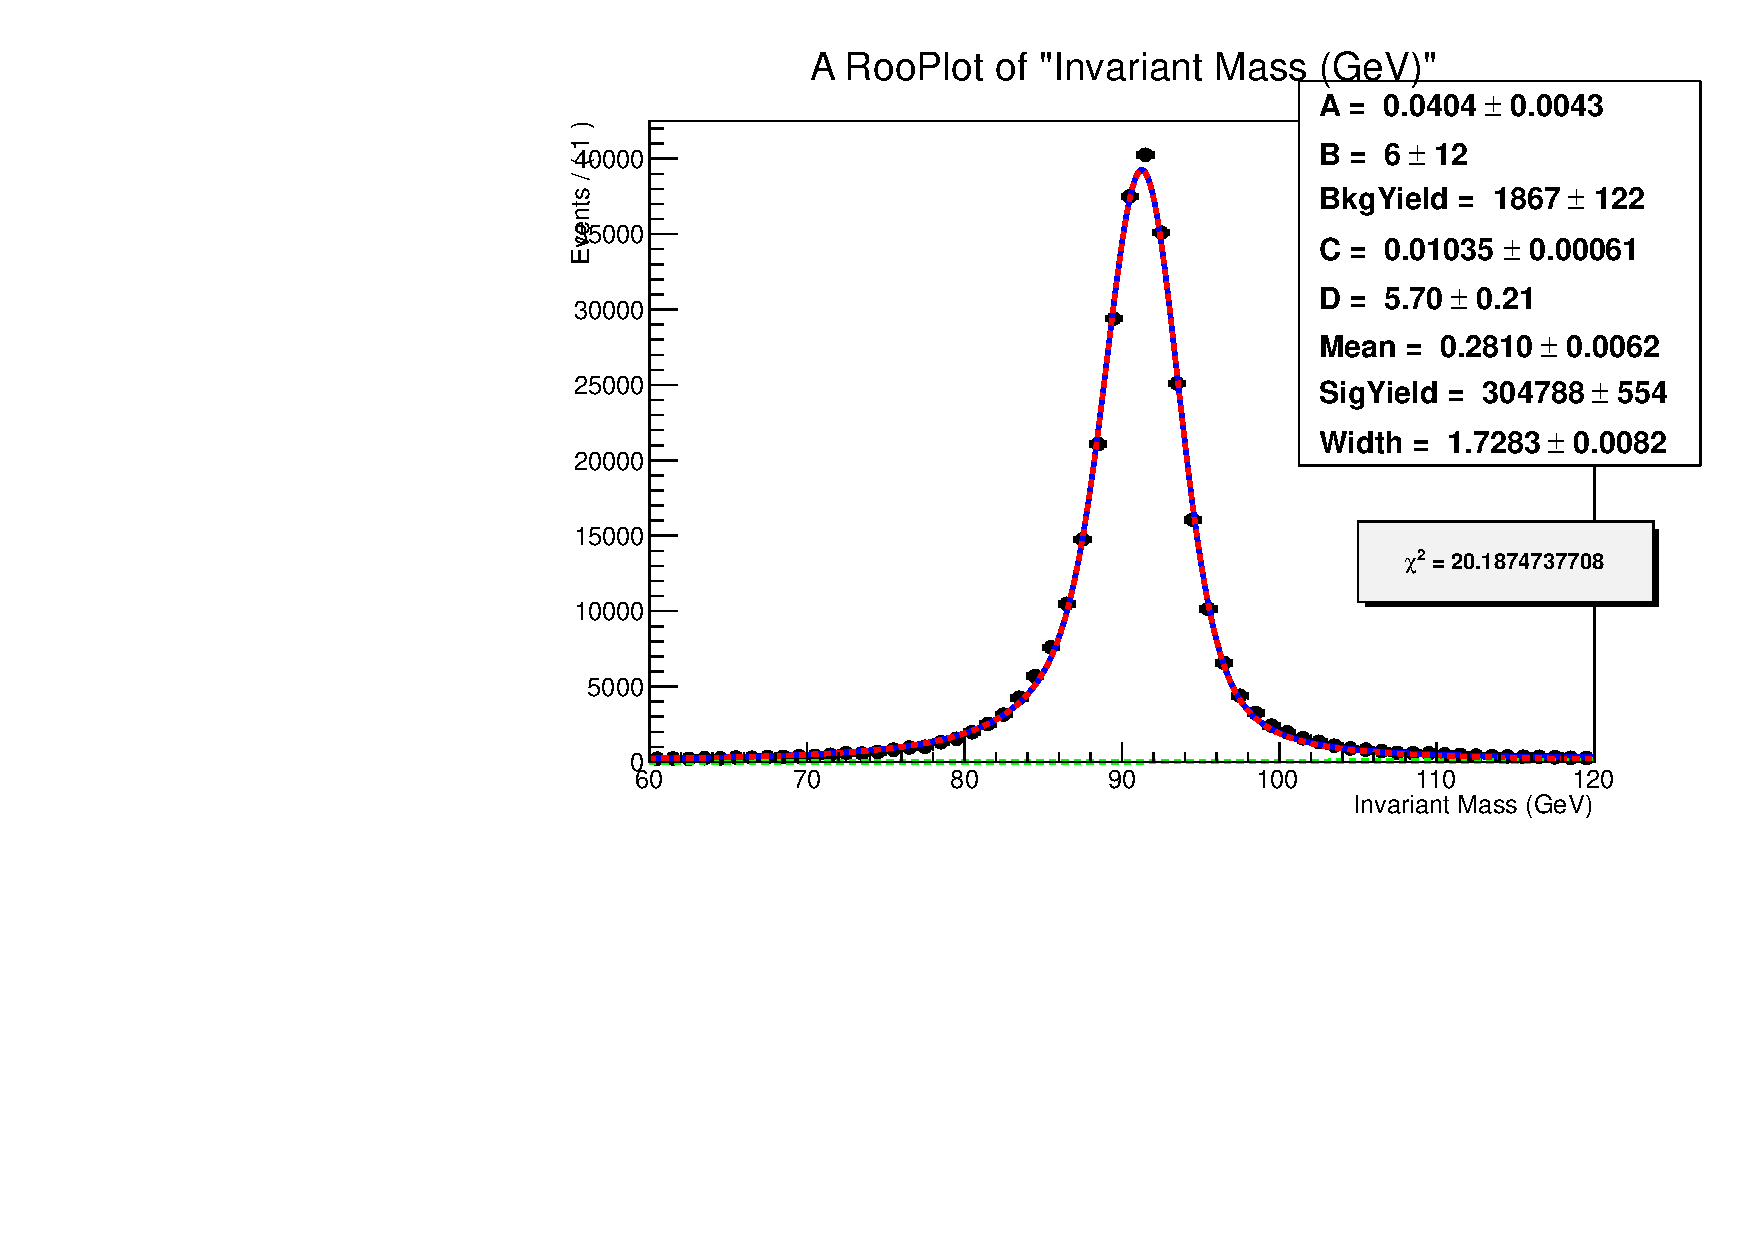
\includegraphics[scale=0.5]{efake_figs/Zek_FullMass.pdf}
%\caption{Fit of the $Z$ invariant mass for the $Z\rightarrow e \gamma_e$ case.}
%\label{Zek}
%\end{center}
%\end{figure}

Assuming a Poissonian error on the signal integral result, the error on the ratio and fake rate can be estimated as:

\begin{eqnarray}
\sigma_R &=& \sqrt{ \frac{1}{N_{e\gamma_e}^2}\sigma_{N_{e\gamma}}^2 + \frac{N_{e\gamma}^2}{N_{e\gamma_e}^4}\sigma_{N_{e\gamma_e}}^2 } \\
\sigma_{FR} &=& \frac{1}{\left( 1 + R \right)^2}\sigma_R.
\end{eqnarray}

With that, we obtain the following results:
\begin{eqnarray}
R &=& \left( 2.38 \pm 0.03 \right)\% \\
F_{e\rightarrow \gamma} &=& \left( 2.32\pm 0.03 \right)\%.
\end{eqnarray}

\subsubsection{Electron $\rightarrow$ Photon Fake Rate Dependencies on \pt, $N_{Vtx}$, $N_{Trk}$}

It has been shown before, in the environment of the SUSY Photon analysis, that the PSV fake rate is dependent on variables such as the probe $p_T$, the number of tracks associated with the primary vertex and the number of reconstructed primary vertices in the event. The nature of the two last dependencies are deeply rooted in the track reconstruction and matching algorithm. 

To check the dependency of the fake rate in the three variables mentioned, the fake rate was calculated in exclusive bins. In each bin, the signal template used was the corresponding bin in the MC signal sample. Each fit was done individually for every bin.

In the plots in Figure \ref{fig:FR_all}, we see how the PSV fake rate depends on the probe $p_T$, number of tracks associated with the primary vertex and the number of reconstructed primary vertices, respectively. The red line in each plot represents the fake rate obtained previously, assuming that there are no dependencies, with the entire invariant mass spectrum. For now on, this first result will be referenced as the flat fake rate.


\begin{figure}[H]
\begin{center}
{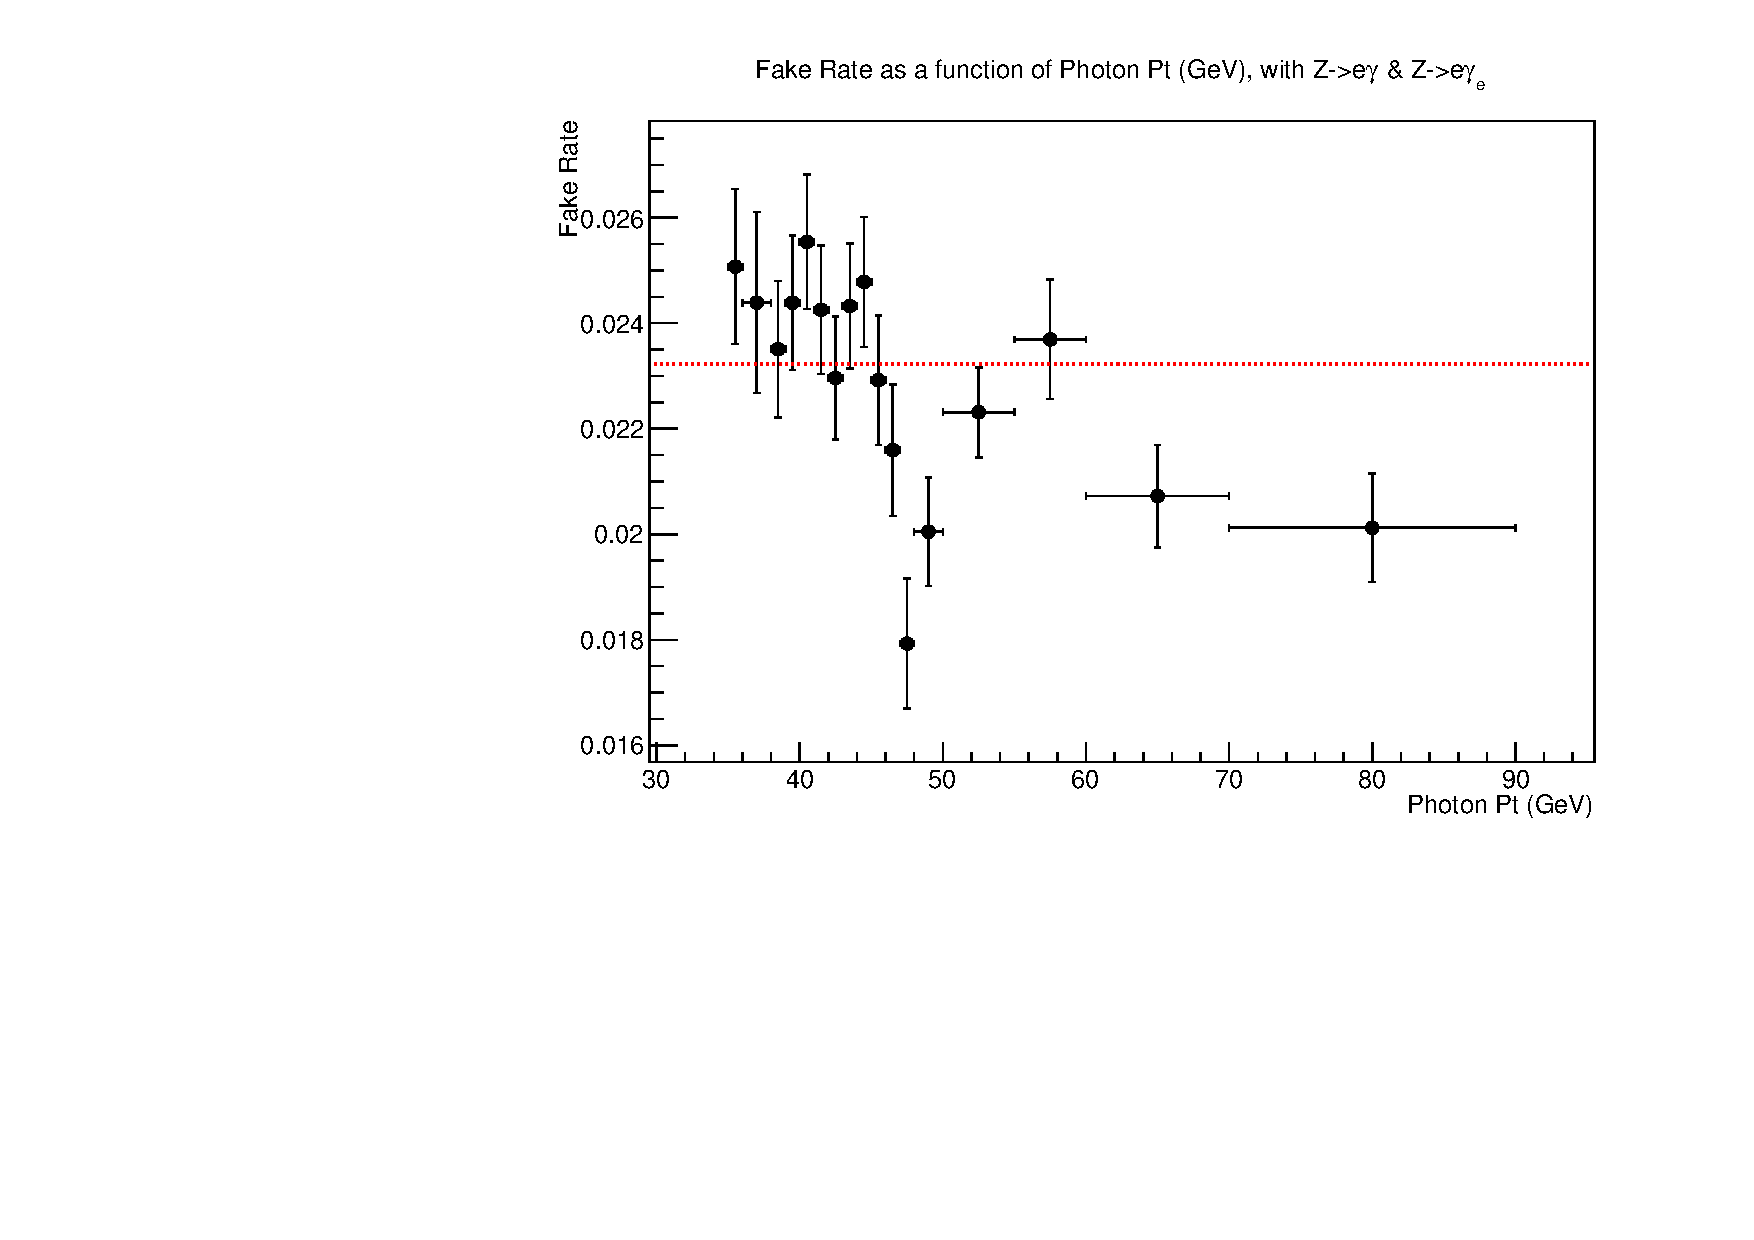
\includegraphics[width=0.45\textwidth]{efake_figs/FakeRate_Pt.pdf}}
{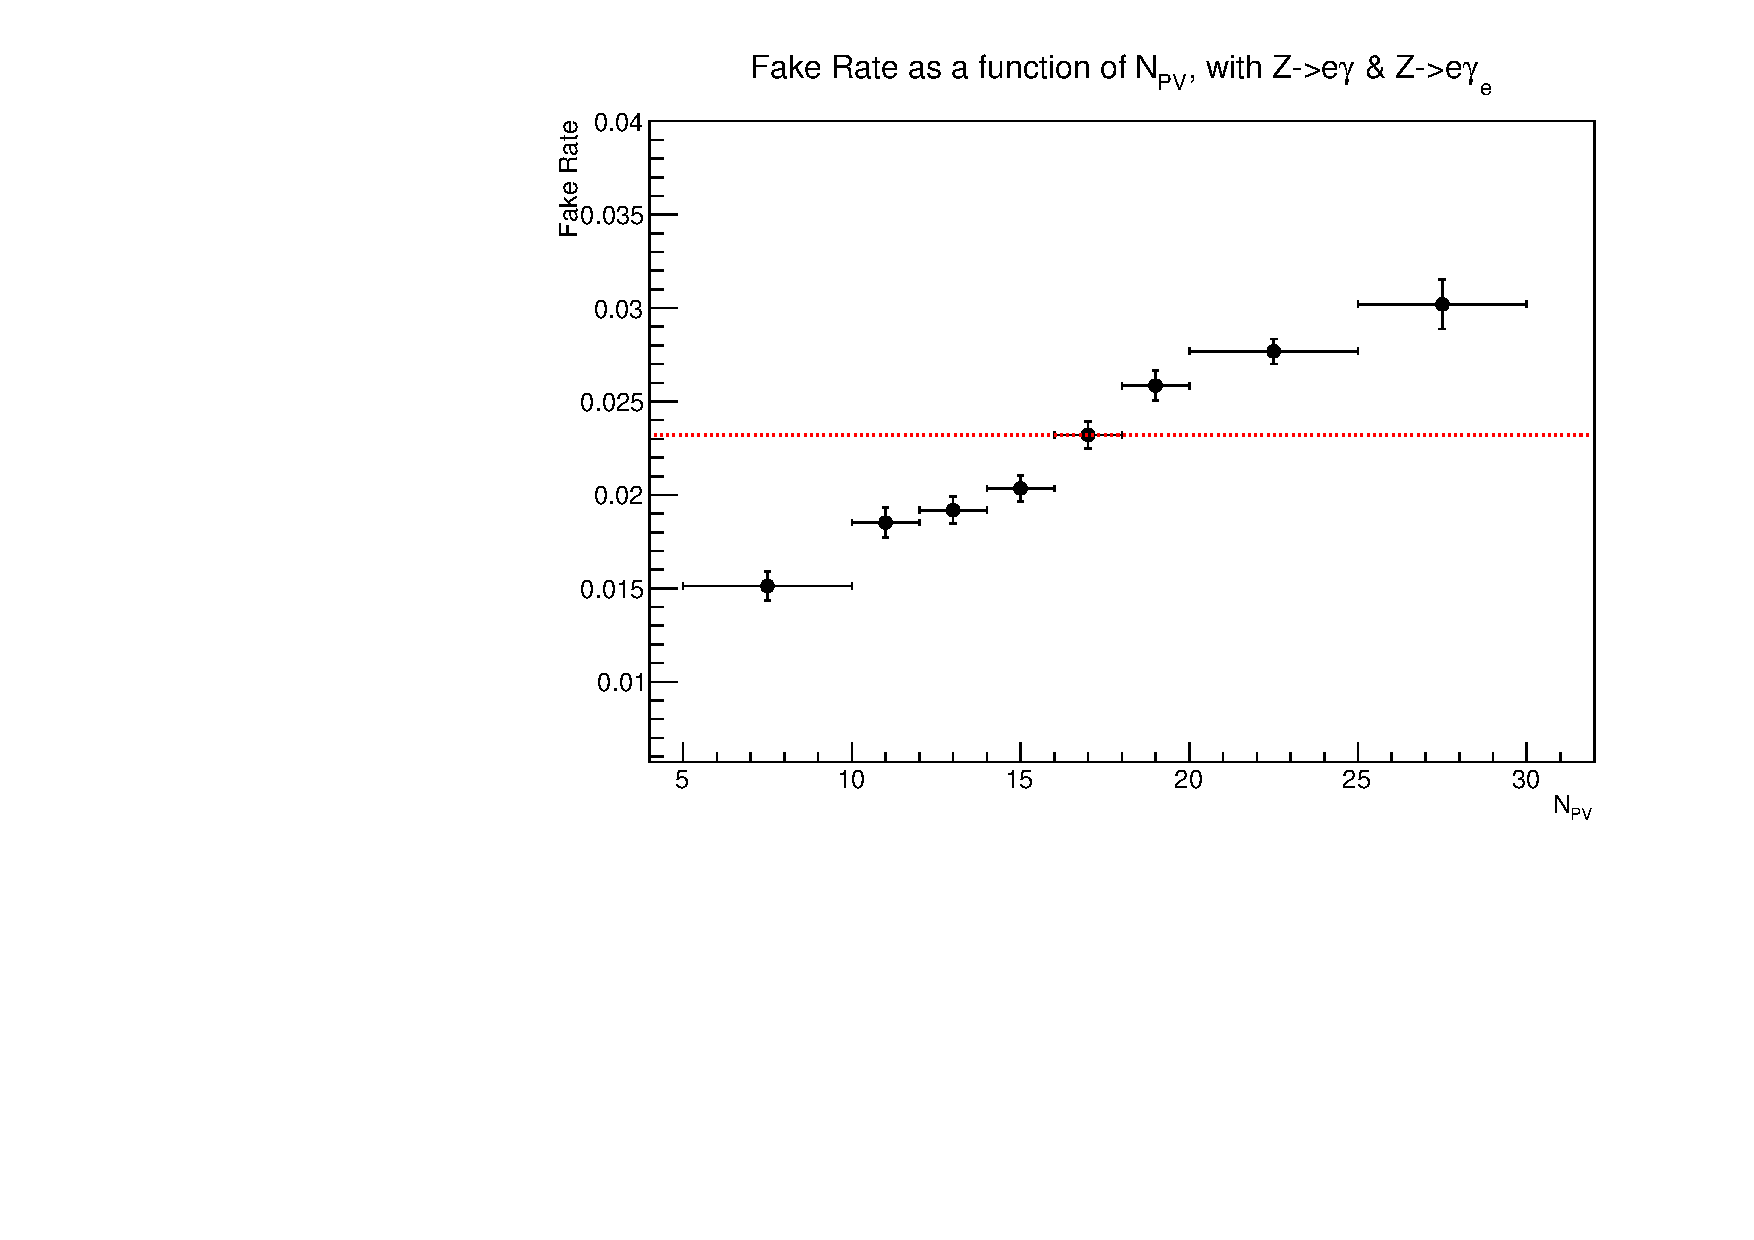
\includegraphics[width=0.45\textwidth]{efake_figs/FakeRate_PU.pdf}}
{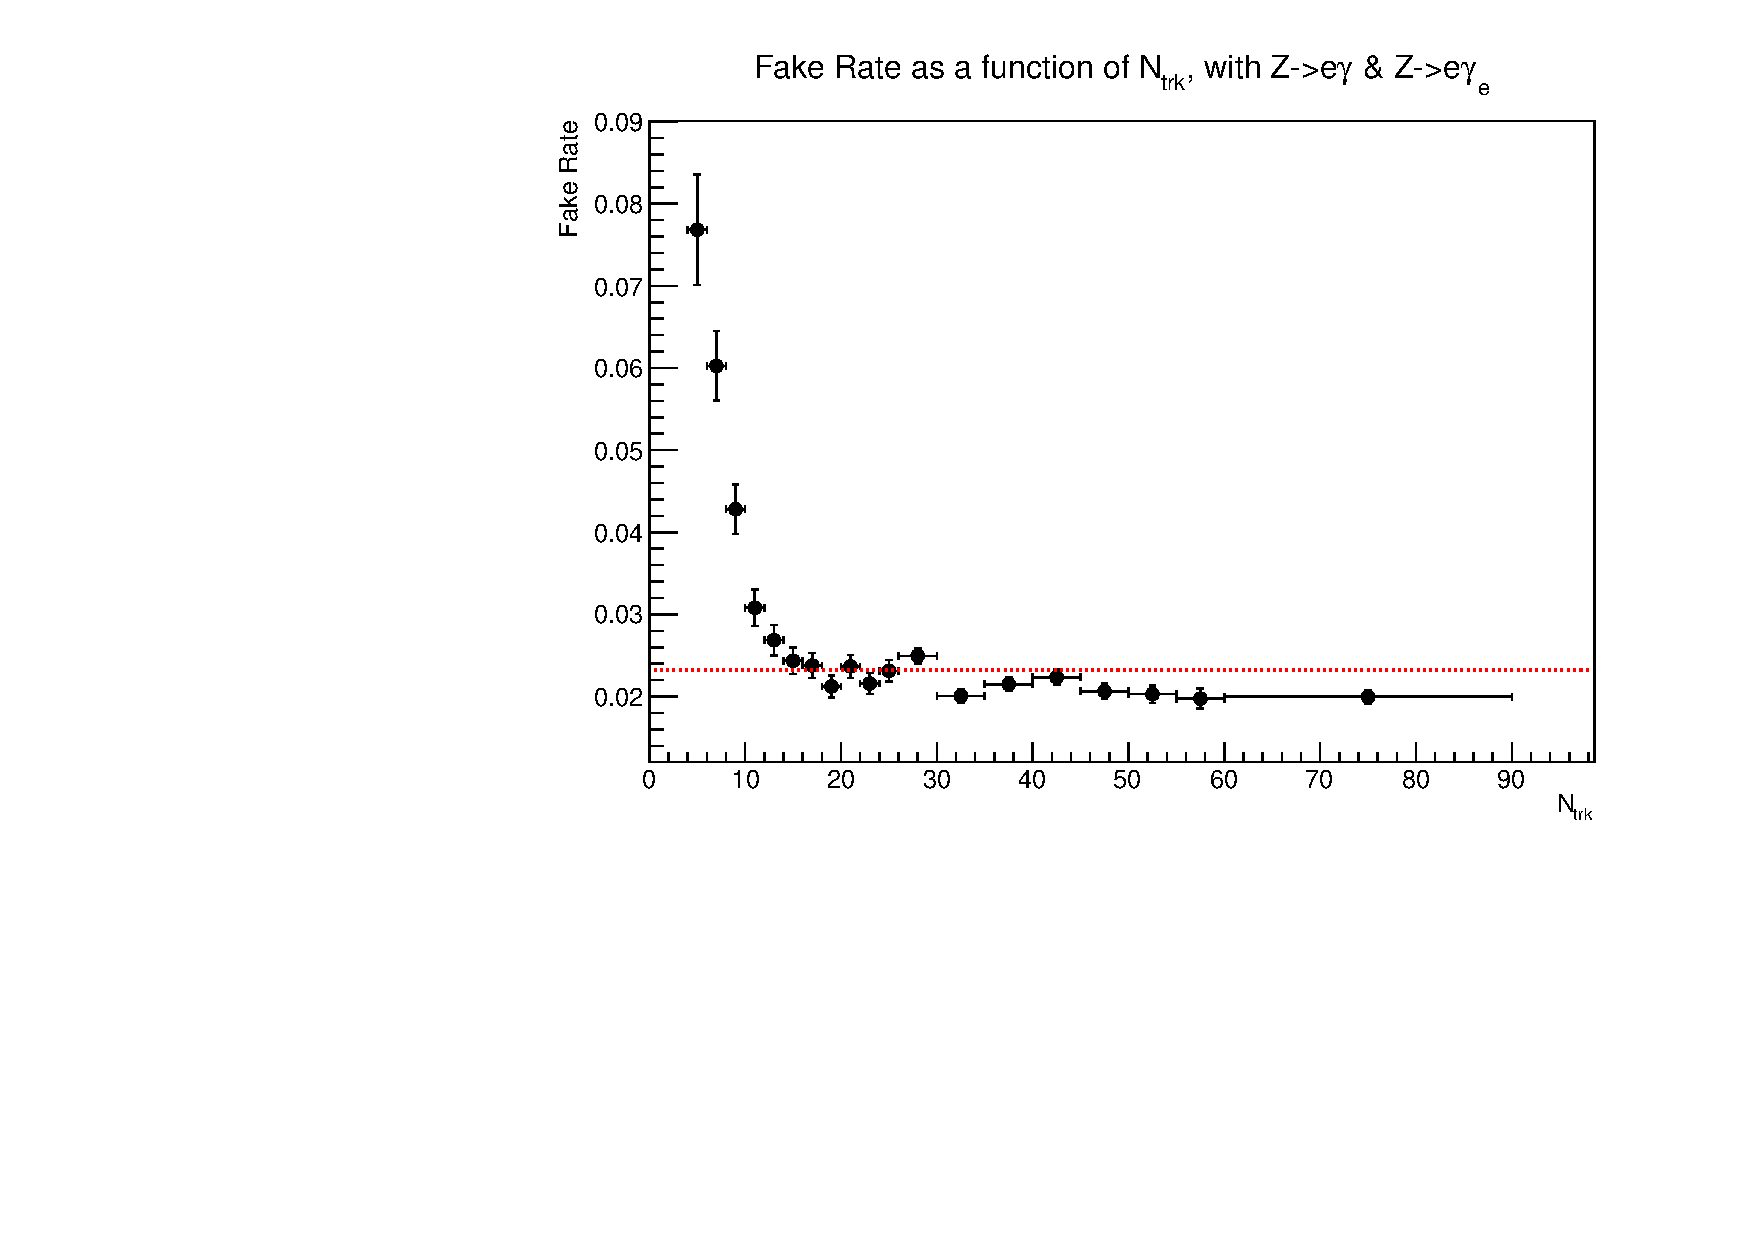
\includegraphics[width=0.45\textwidth]{efake_figs/FakeRate_Trk.pdf}}
\caption{Fake rate vs. probe $p_T$, number of primary vertices and track multiplicity.}
\label{fig:FR_all}
\end{center}
\end{figure}

As shown in the plots, there is a non-trivial dependency of the fake rate on the variables probed. There are different ways to solve this feature. The most complete one would be to achieve a multi-parameter description of the fake rate, including a 3-dimensional function with dependencies of the fake rate on each variable. That, however, demands a thorough study of these dependencies and a functional form to perform this task. A second way would be to choose one of the parametrizations, including the flat one, and prescribe a systematical error to that assumption. To know how much one choice impacts the fake rate, we can look at the final result and observe how much the yields change with each assumption.

In our case, the final result is the control sample of photon-like objects that fail the pixel seed veto normalized by the fake rate, which represents the estimation of our electron faking photon contamination in the signal region. The plots in Figure \ref{CS_params} show the shape and yields of this control sample when normalized by the different parametrizations of the fake rate. When checking the differences in number of events of each bin, we see that they are all within $5\%$ of each other, being higher around the $p_T$ peak and approaching $0$ for higher values. Therefore, it is safe to choose any specific parametrization and assume a systematic error of $5\%$ on the number of events to make sure that the different assumptions are compatible. With these assumptions, we choose to use the flat parametrization, since it only involves one fit and it has been shown to be much more stable with respect to different fit functions, for signal and background.


\begin{figure}[H]
\begin{center}
  {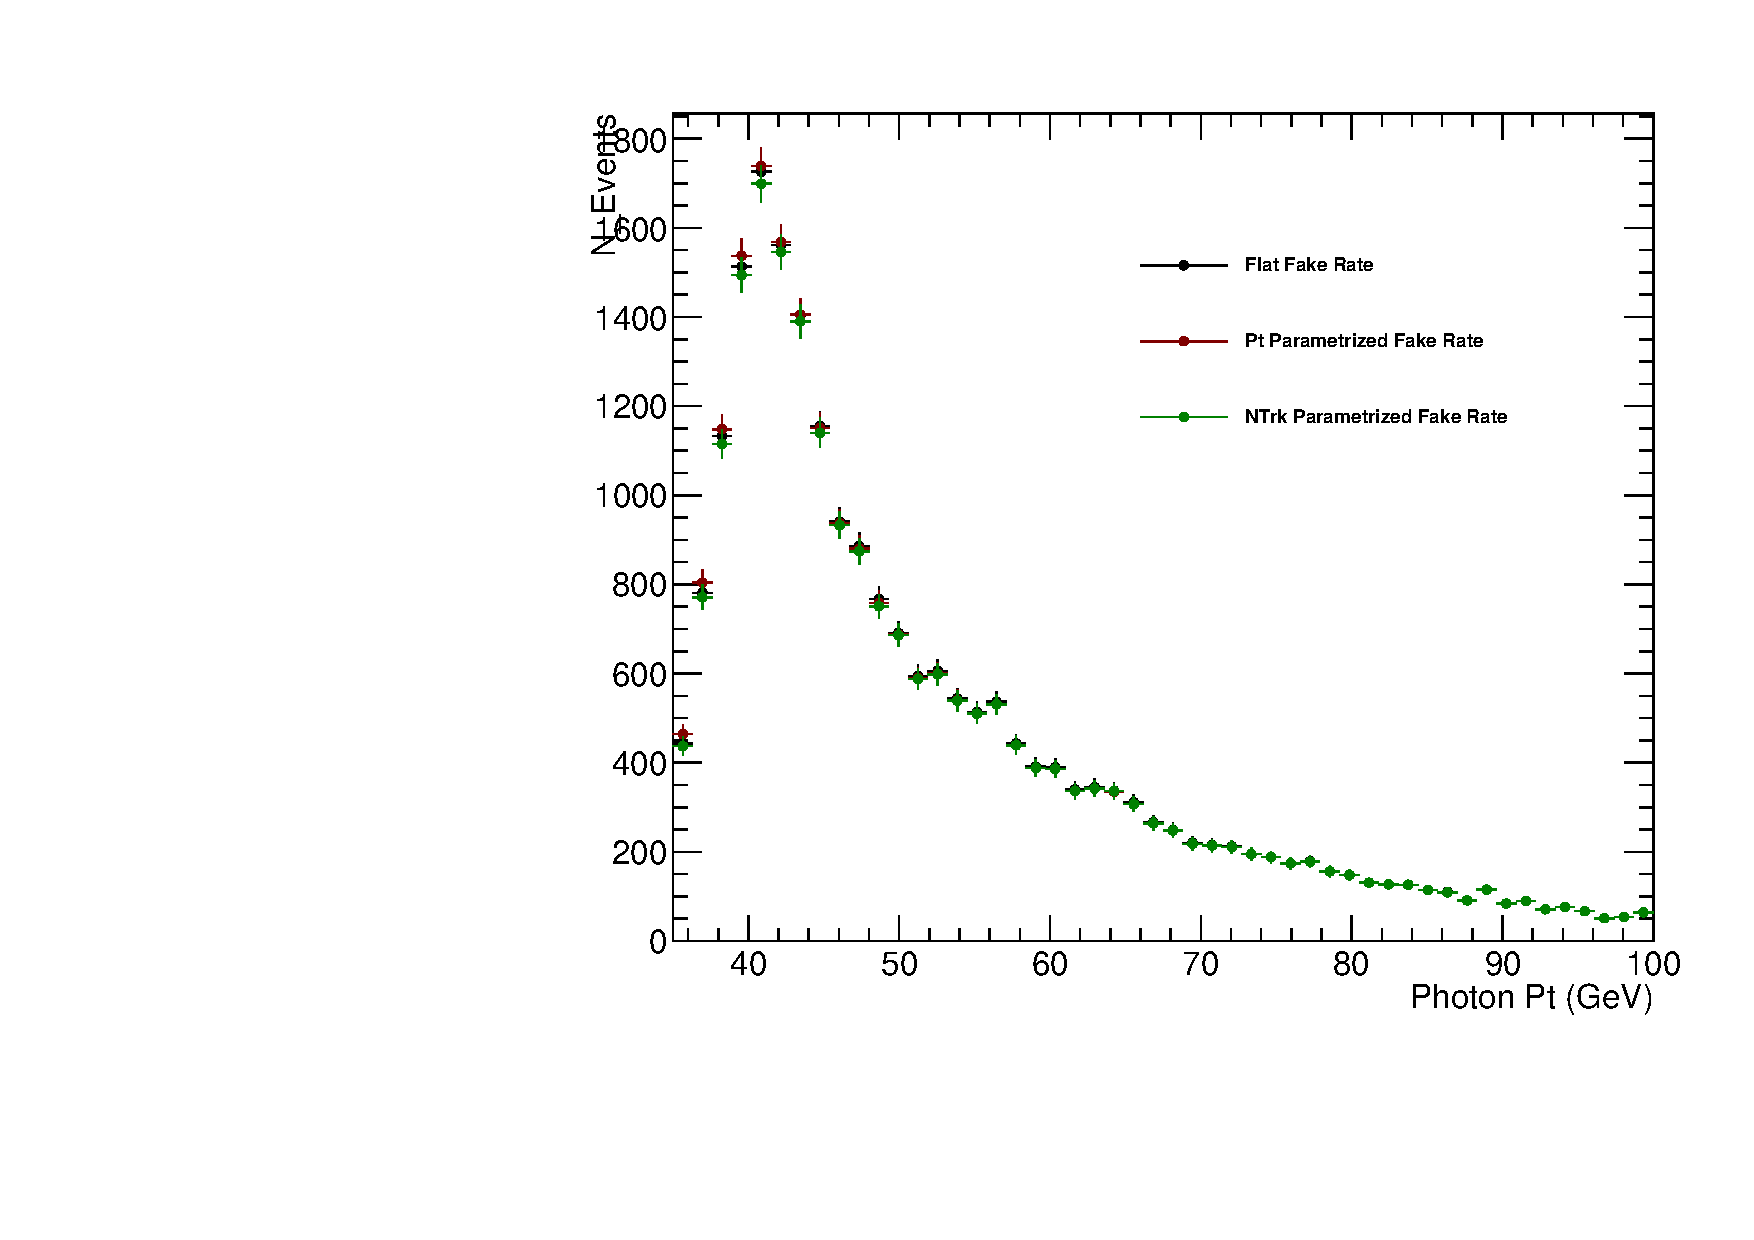
\includegraphics[width=0.45\textwidth]{efake_figs/CS_param_pt.pdf}}
  {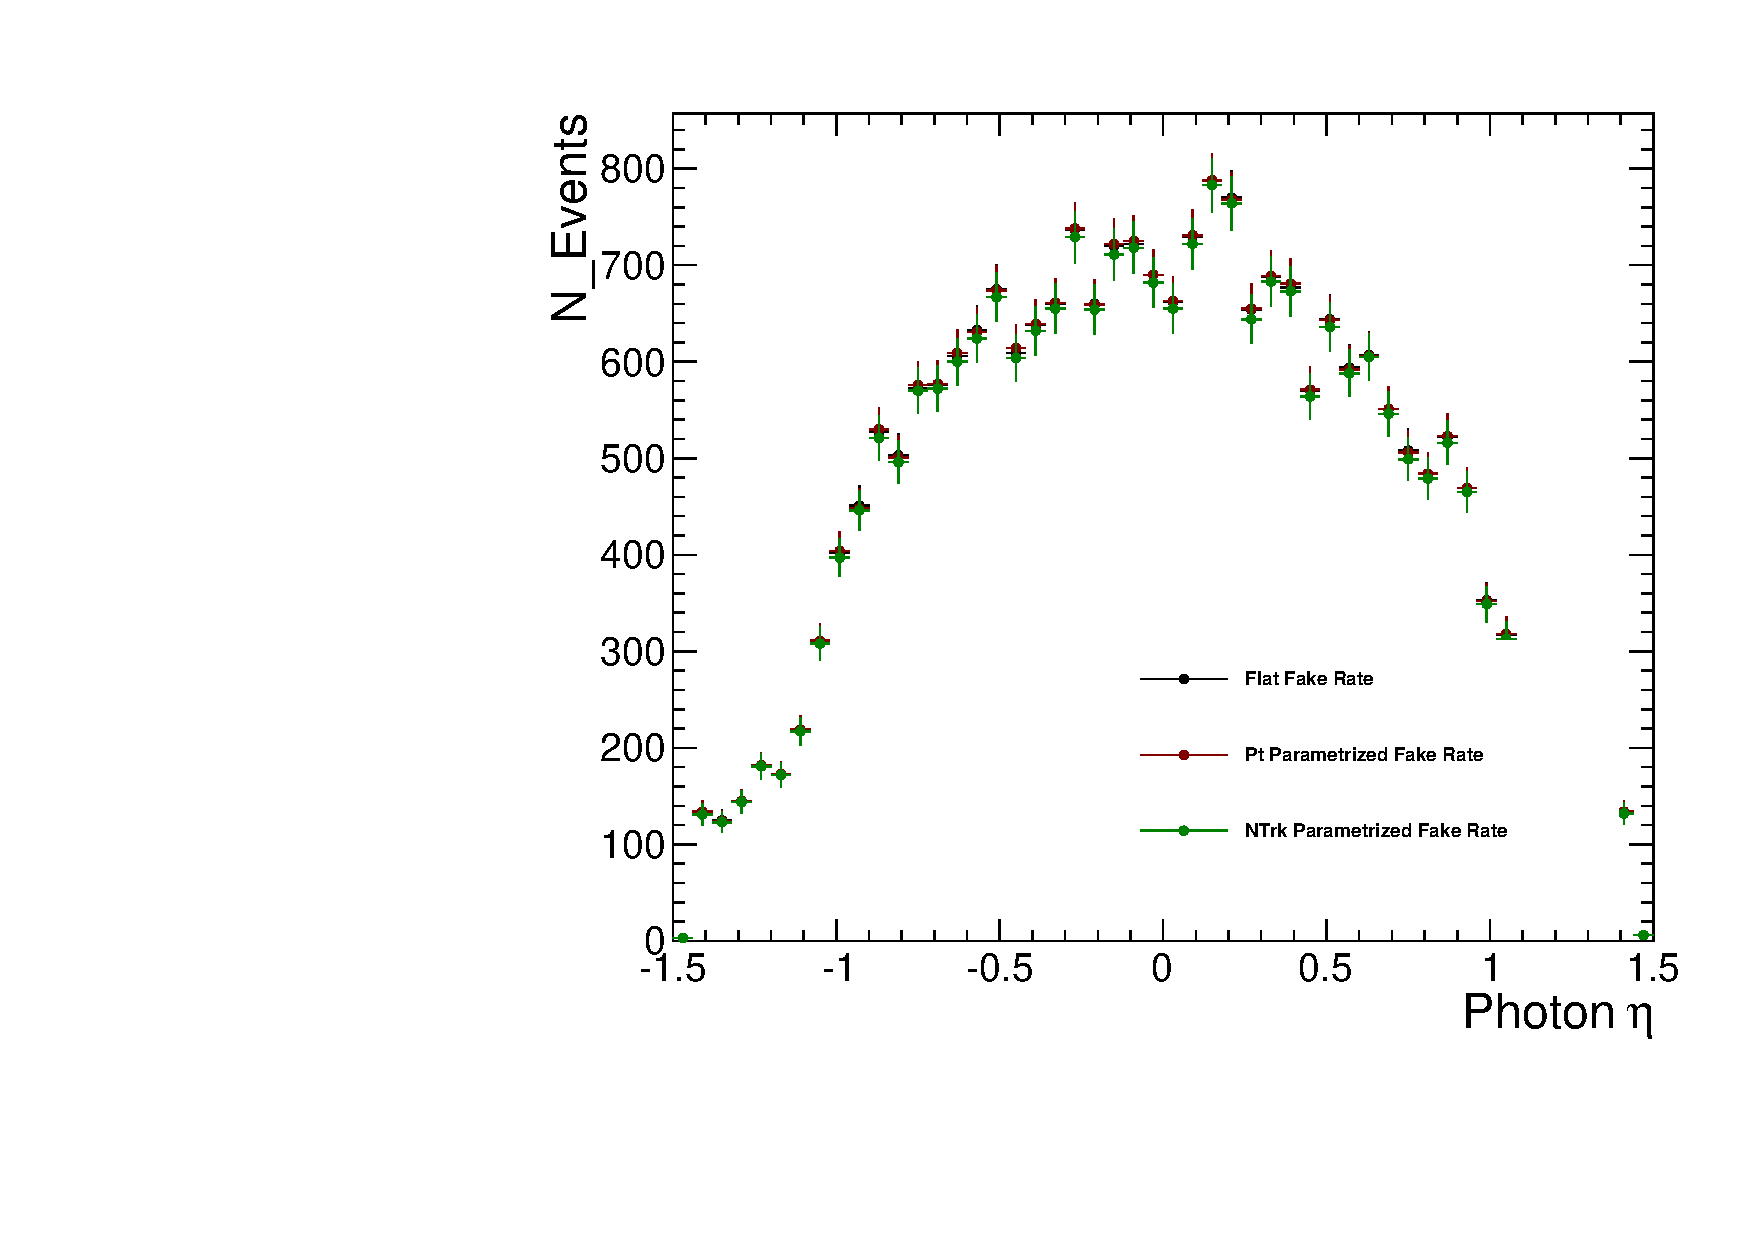
\includegraphics[width=0.45\textwidth]{efake_figs/CS_param_eta.pdf}}
\\
  {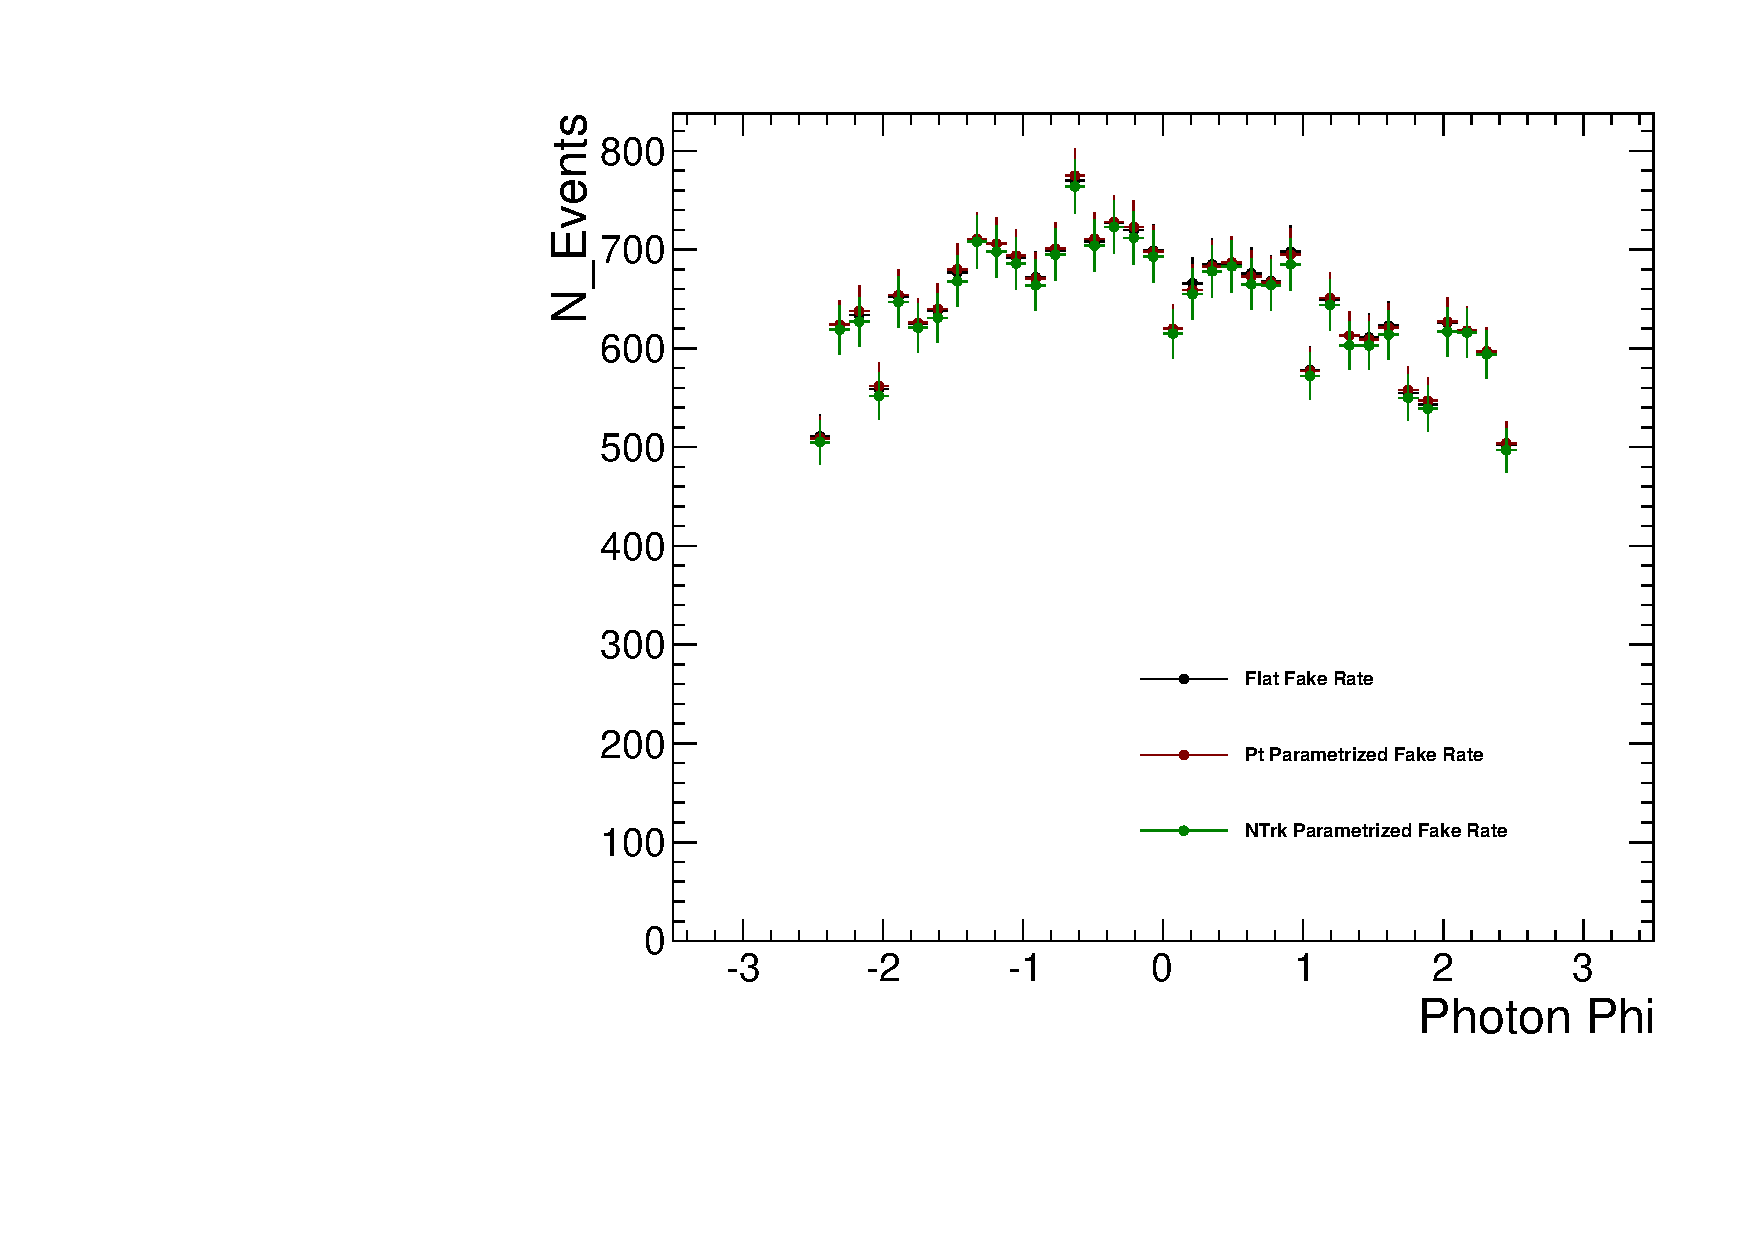
\includegraphics[width=0.45\textwidth]{efake_figs/CS_param_phi.pdf}}
\caption{Control sample distribution of photon $p_T$, $\eta$ and $\phi$.}
\label{CS_params}
\end{center}
\end{figure}

\subsubsection{Closure Test for Electron $\rightarrow$ Photon Fake Rate Measurment}

As a closure test, we compare the generator-level fake rate to the fake rate as calculated by the method described above on MC (the reco-level fake rate) and check that they agree.
%To make sure the method makes sense, we have to test whether or not it closes on Monte Carlo. That means that we have to compare the generator-level fake rate to the method fake rate on Monte Carlo and make sure that they agree. 
For that, we used the Drell-Yan sample.

The generator-level fake rate is defined as:

\begin{eqnarray}
F_{gen} = \frac{\textrm{\#Medium ID Photons \&\& Matched to Gen Electrons \&\& Pass the PSV}}{\textrm{\#Medium ID Photons \&\& Matched to Gen Electrons}}. \label{gen_fake}
\end{eqnarray}

Here, the Medium photon ID is the one used on the analysis, including all the shower shape cuts to remove spikes and other contributions.

We compare the results of the two measurements, generator-level and reco-level, on the plots in Figure \ref{closure_old}.

\begin{figure}[H]
\begin{center}
{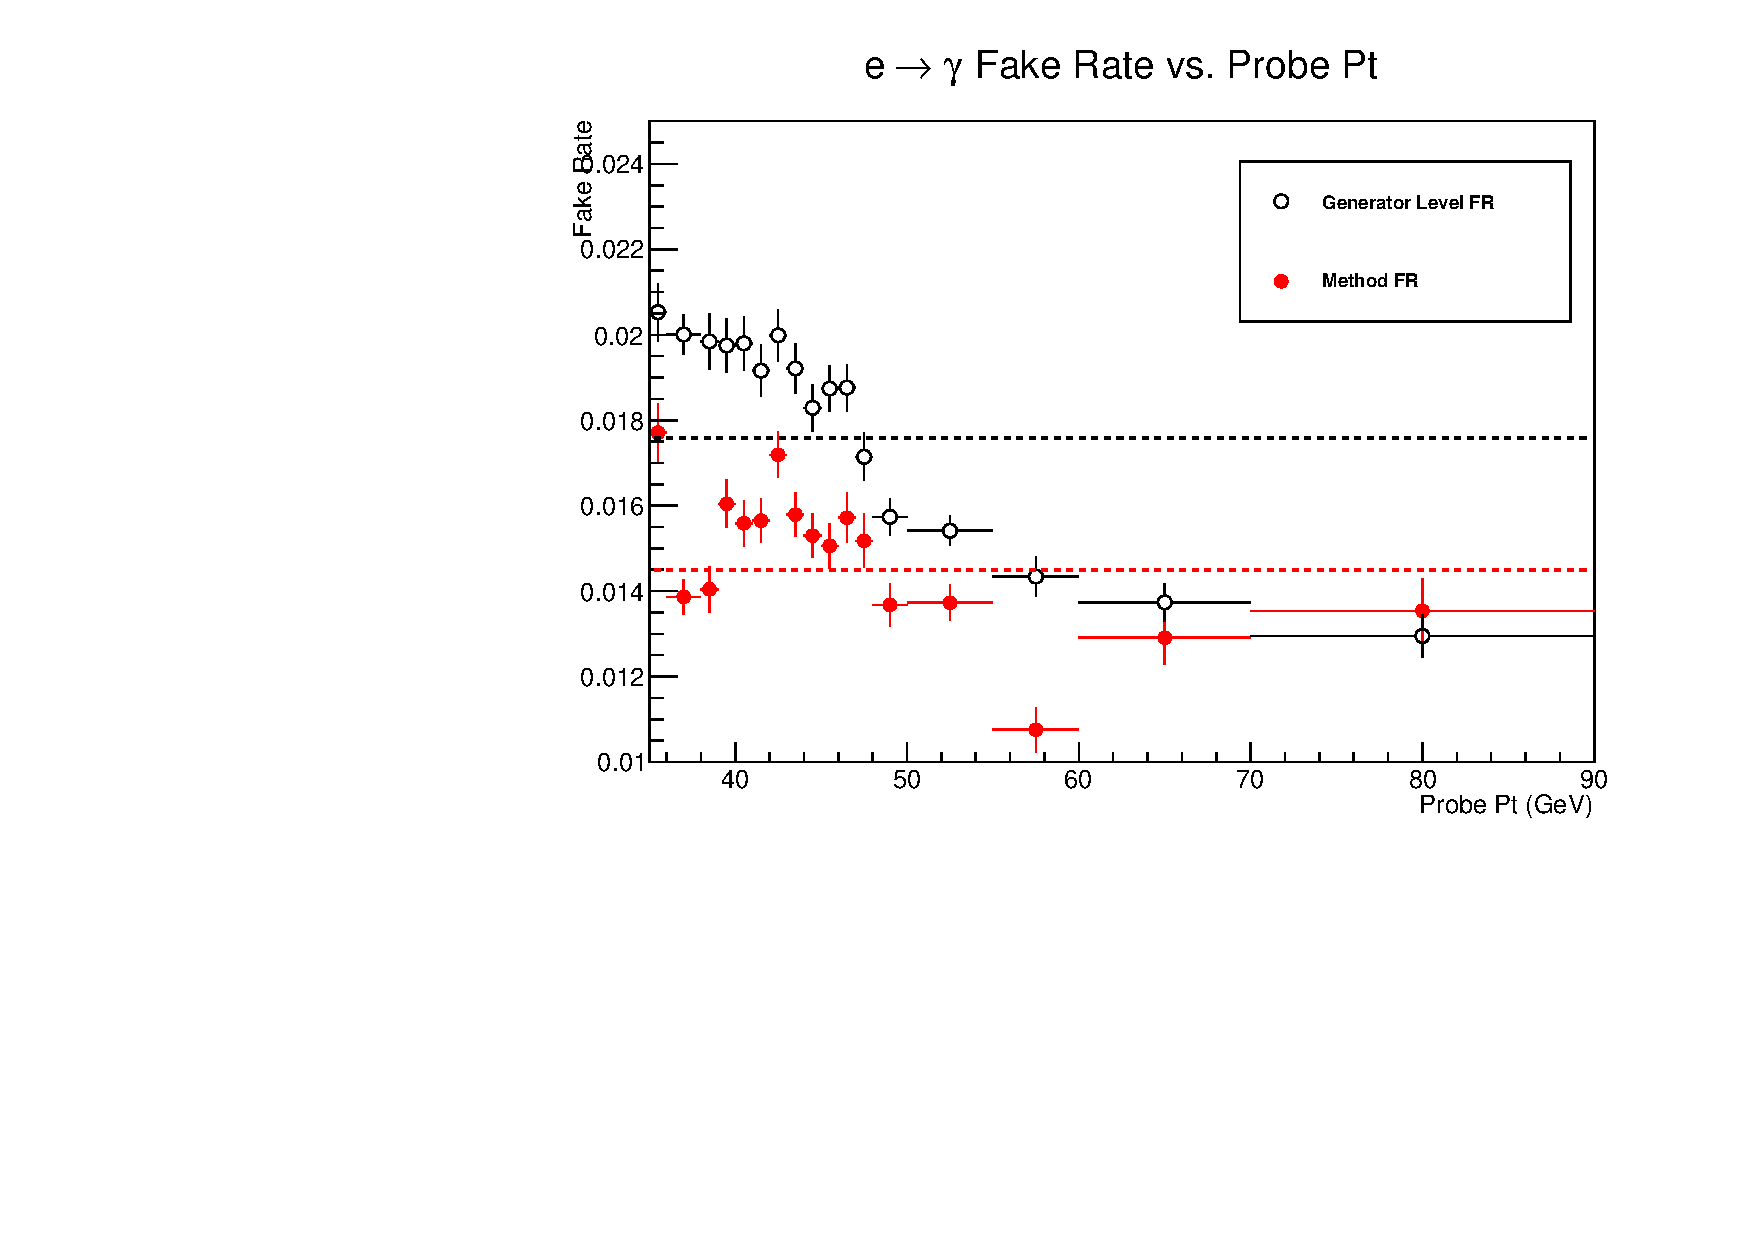
\includegraphics[width=0.45\textwidth]{efake_figs/closure_old_pt.pdf}}
{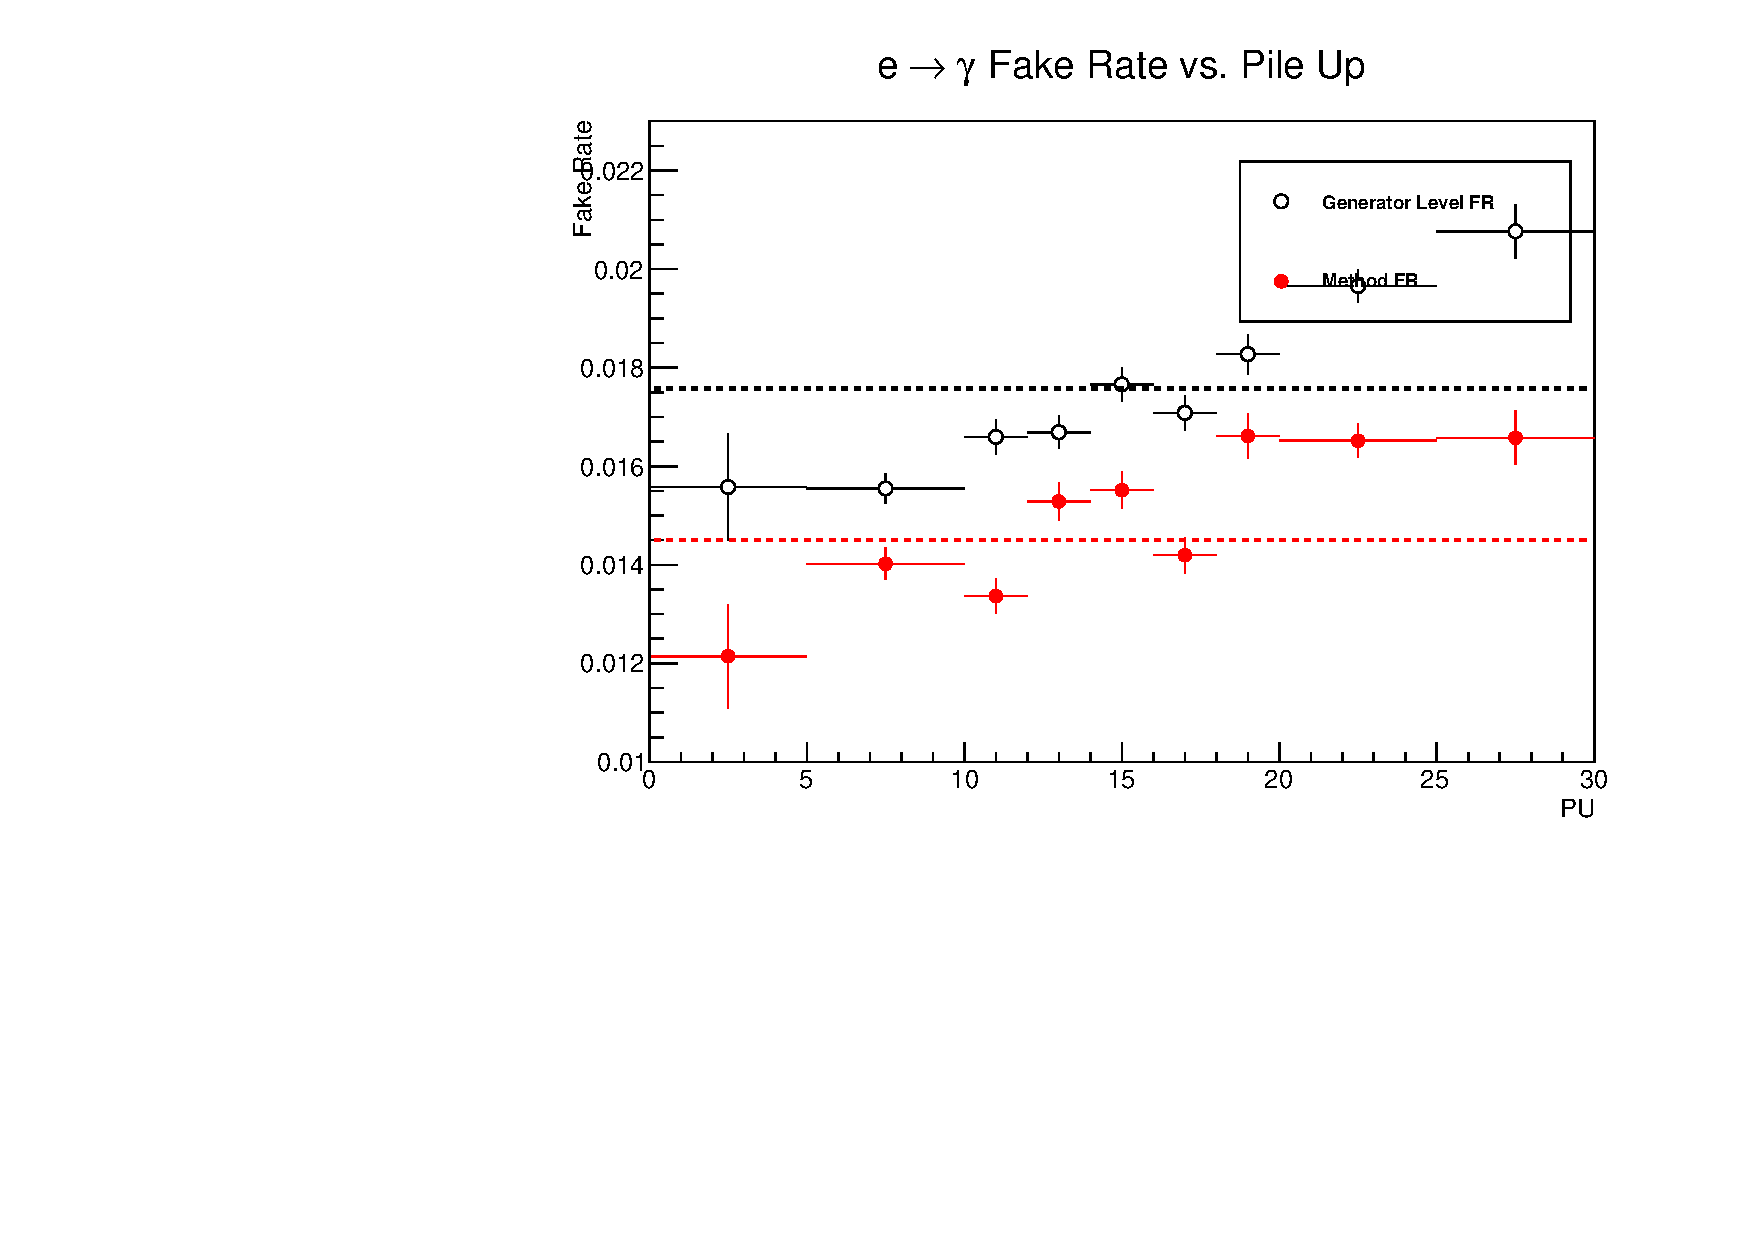
\includegraphics[width=0.45\textwidth]{efake_figs/closure_old_pu.pdf}}
\\
{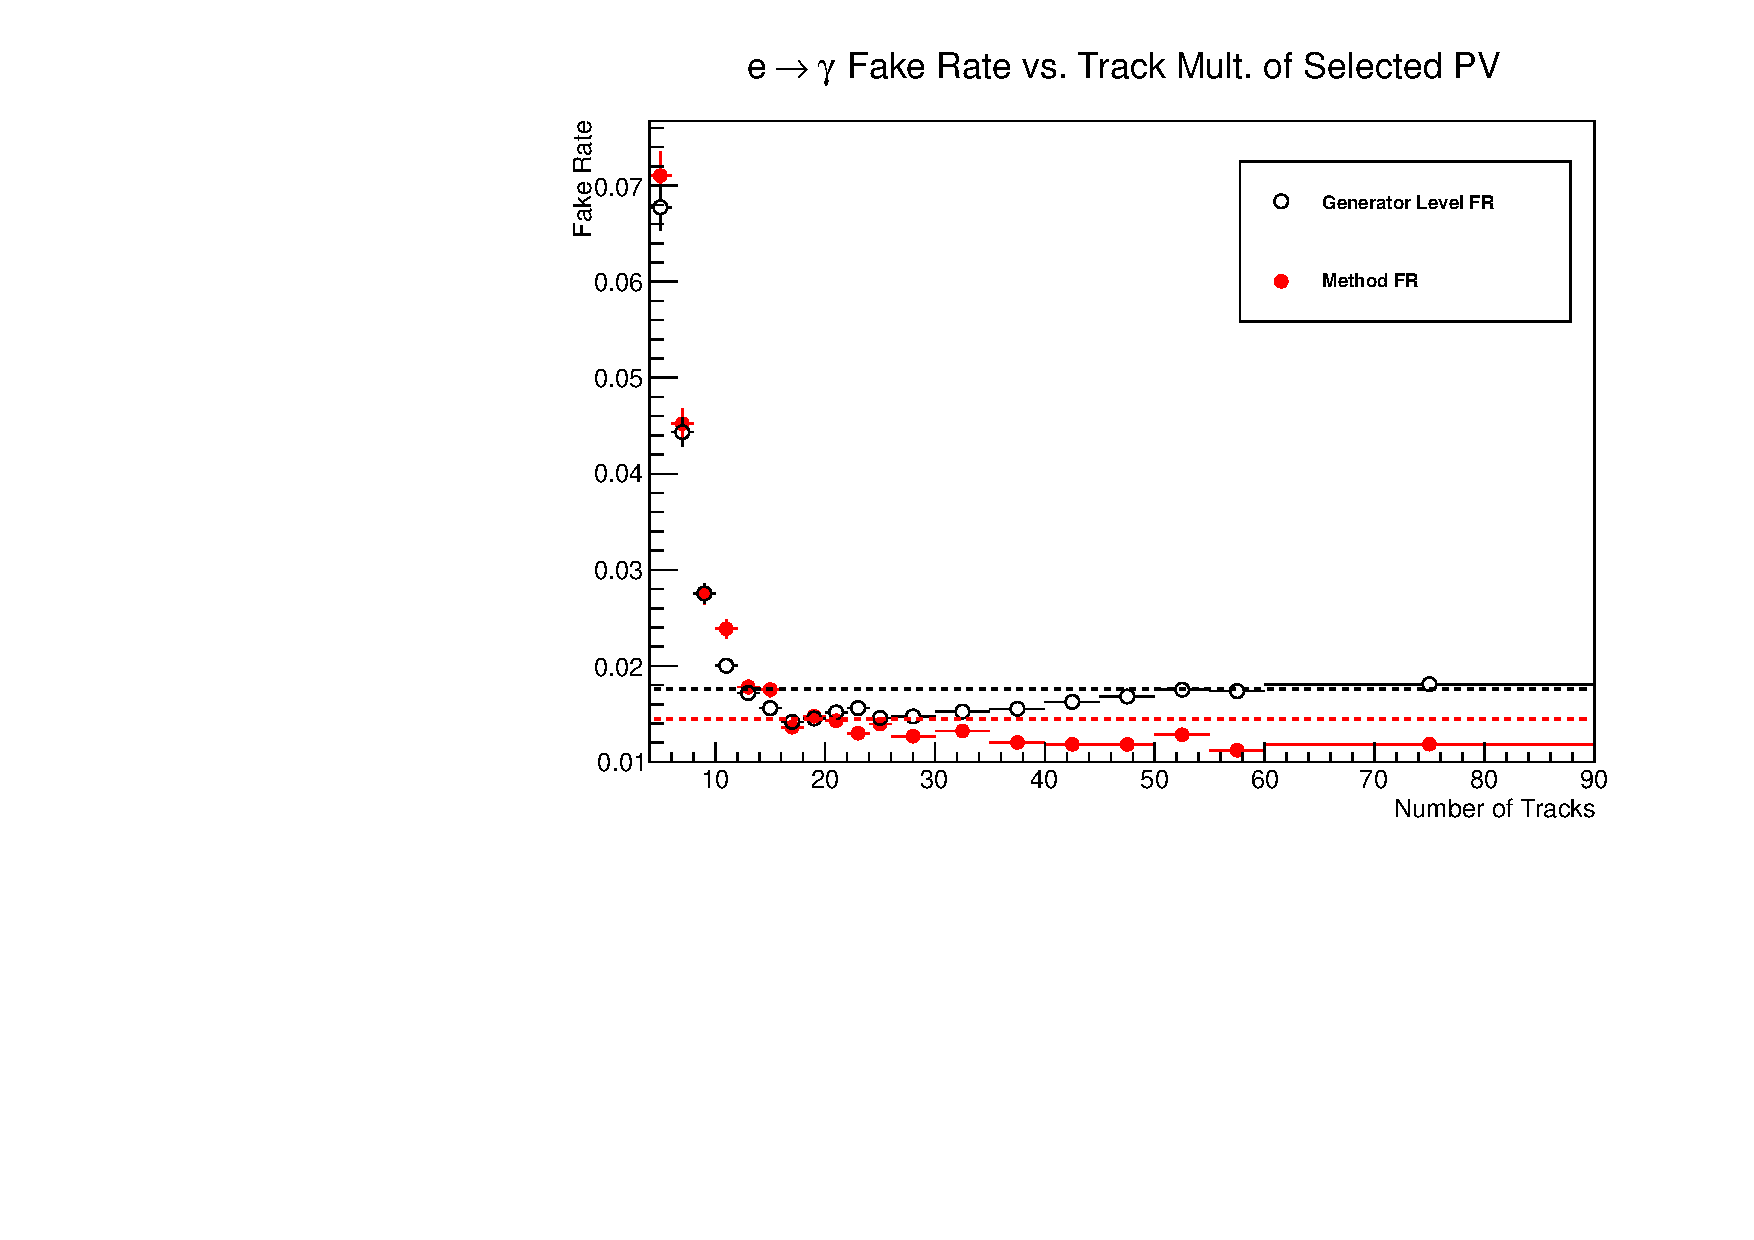
\includegraphics[width=0.45\textwidth]{efake_figs/closure_old_trk.pdf}}
\caption{Closure test in probe $p_T$,number of reconstructeed primary vertices and track multiplicity .}
\label{closure_old}
\end{center}
\end{figure}
%
%\begin{figure}[H]
%\begin{center}
%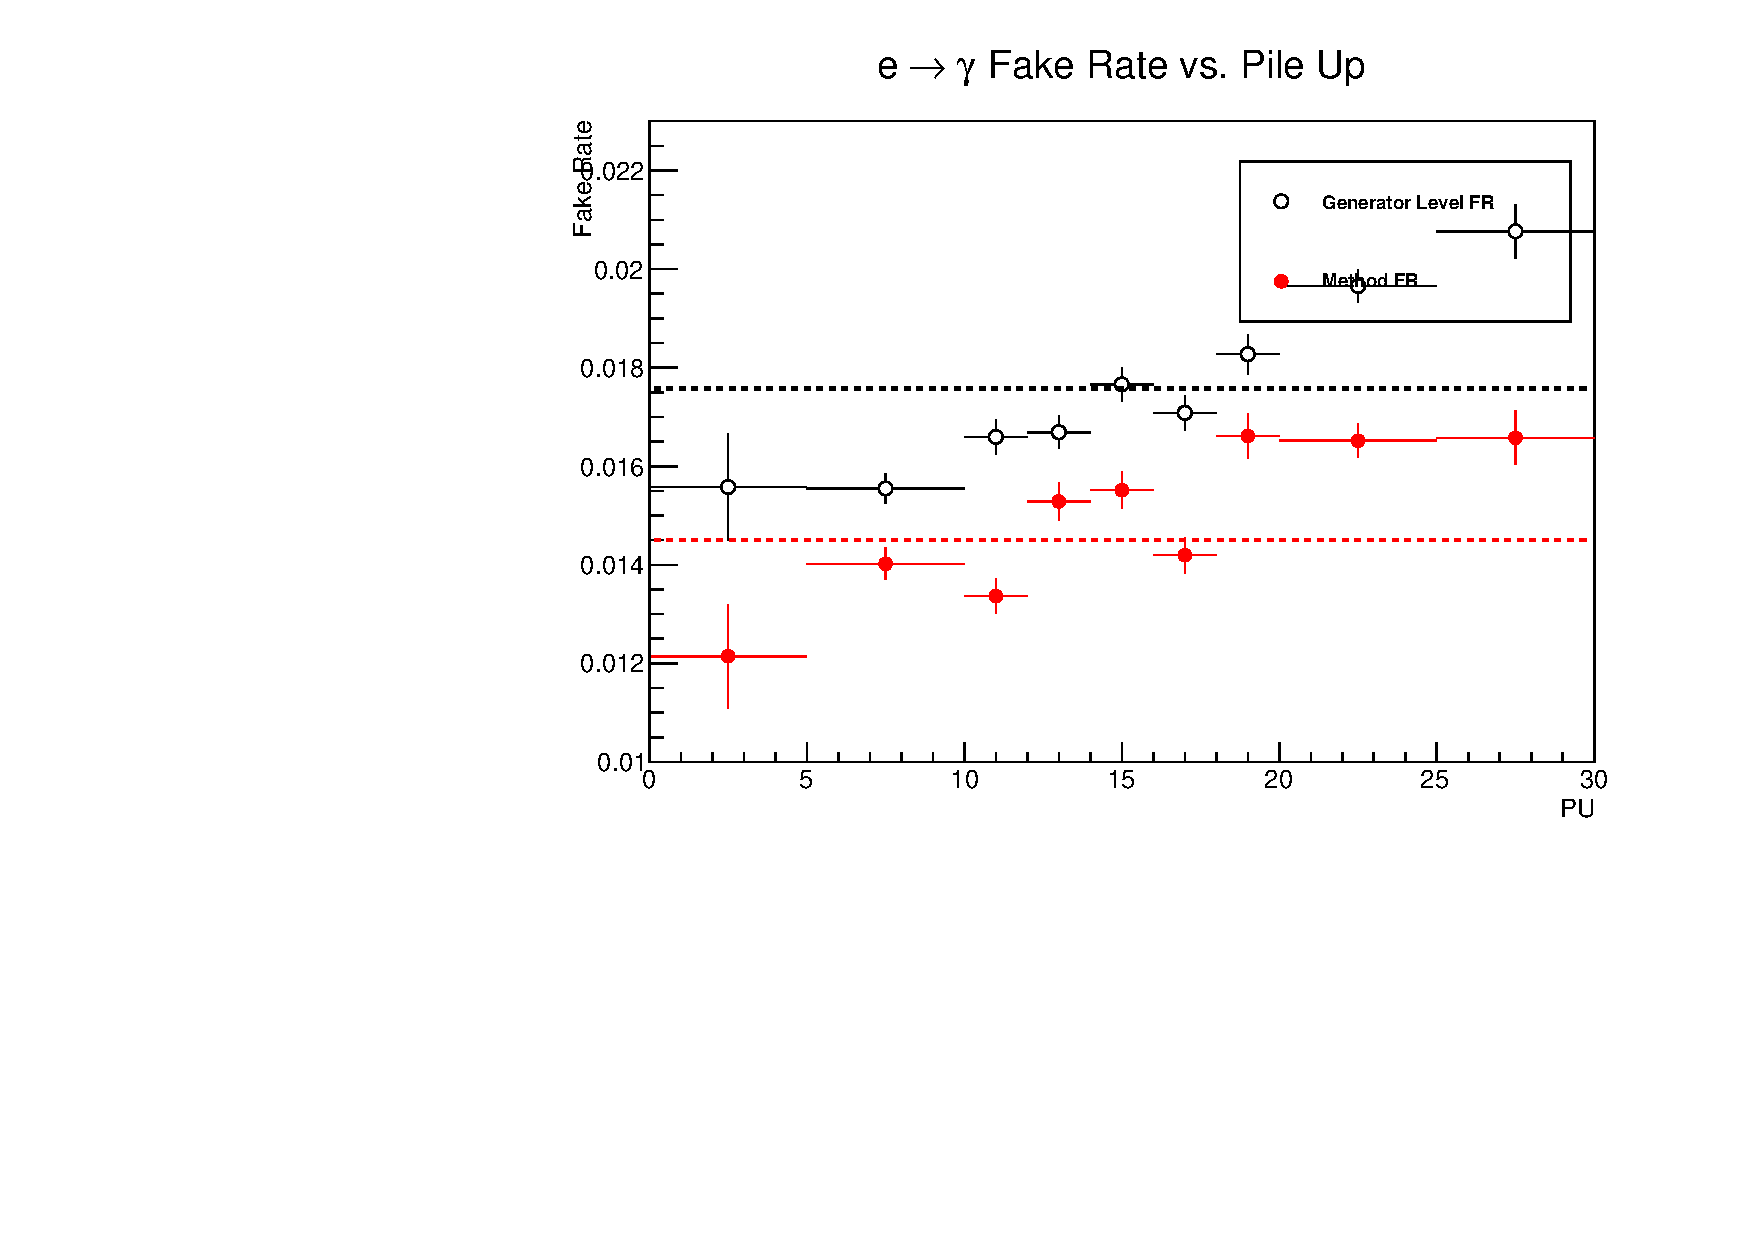
\includegraphics[scale=0.5]{efake_figs/closure_old_pu.pdf}
%\caption{Closure test in number of reconstructeed primary vertices.}
%\label{closure_old_pu}
%\end{center}
%\end{figure}

%\begin{figure}[H]
%\begin{center}
%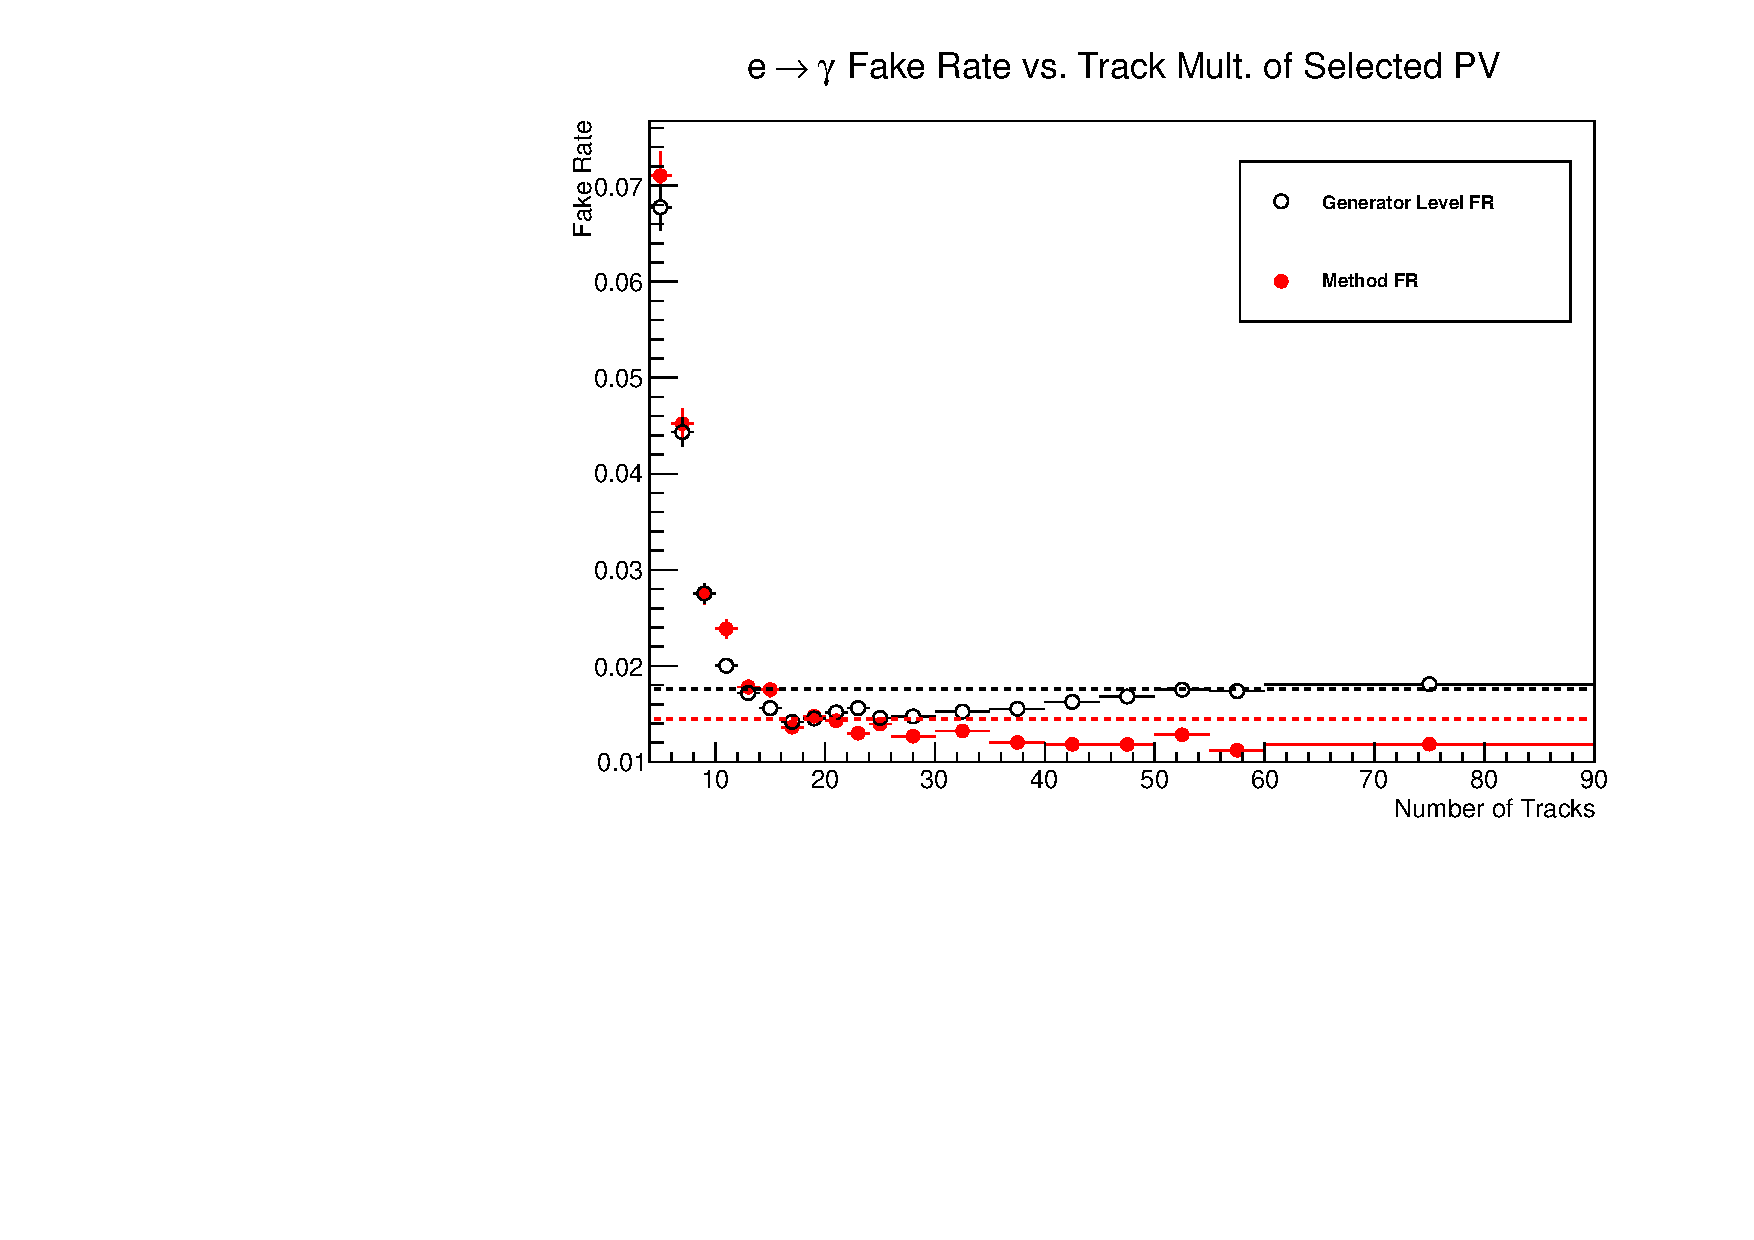
\includegraphics[scale=0.5]{efake_figs/closure_old_trk.pdf}
%\caption{Closure test in track multiplicity.}
%\label{closure_old_ntrk}
%\end{center}
%\end{figure}

The lines represent the fake rate results from the flat assumption. For the generator-level fake rate, that is just the ratio on equation \ref{gen_fake} on all events, while the parametrized fake rate is the ratio in each bin. As shown, there is a significant discrepancy between the two measurements. With those results, we can only say that the method is closed within 20\%. The 20\% number comes from the difference between the flat fake rates on generator-level and reco-level results.

We investigated the cause of this result and noticed that it comes about because of a "hidden" primary vertex matching on the tag-and-probe method. When using the tag and probe for electrons as tag and photons as probe, the photon ends up being matched to the hardest primary vertex because the electron, in the electron ID requirements, is indeed matched. When we require the invariant mass of the pair to be close to the $Z$ peak, the electron PV matching is indirectly passed to the probe photon, since they must come from the same source. This requirement does not exist on the gen-level fake rate, which is basically a counting experiment.

The importance of the PV matching requirement comes about because of the nature of the DY$\to ee$ process. Since it is a low multiplicity process, i.e., there will not be many objects naturally from the hard scatter process, the $Z$ might not come from the hardest reconstructed primary vertex of the event. Therefore, when that happens, we measure the fake rate from a  primary vertex that is not the hardest and, therefore, has fewer tracks than the primary vertex assumed. Since we know that the fake rate increases sharply when there are few tracks in the primary vertex, that explains why, in plot \ref{closure_old}, there is an increase in higher values of NTrack - those are actually hard scatter events with few tracks that were mistakenly matched to the hardest PV.

To overcome these problems, we match the gen-level particles used for the gen-level fake rate to the hardest reconstructed primary vertex with the following cuts (from the muon ID POG recommendations):

\begin{itemize}
\item $Dz < 0.5$;
\item $Dxy < 0.2$.
\end{itemize}

These variables are obtained directly from methods of the RECO::Candidate class inherited by the RECO::GenParticle.
With that, we have the plots on Figure \ref{closure_all}.

\begin{figure}[H]
\begin{center}
{\label{closure_pt}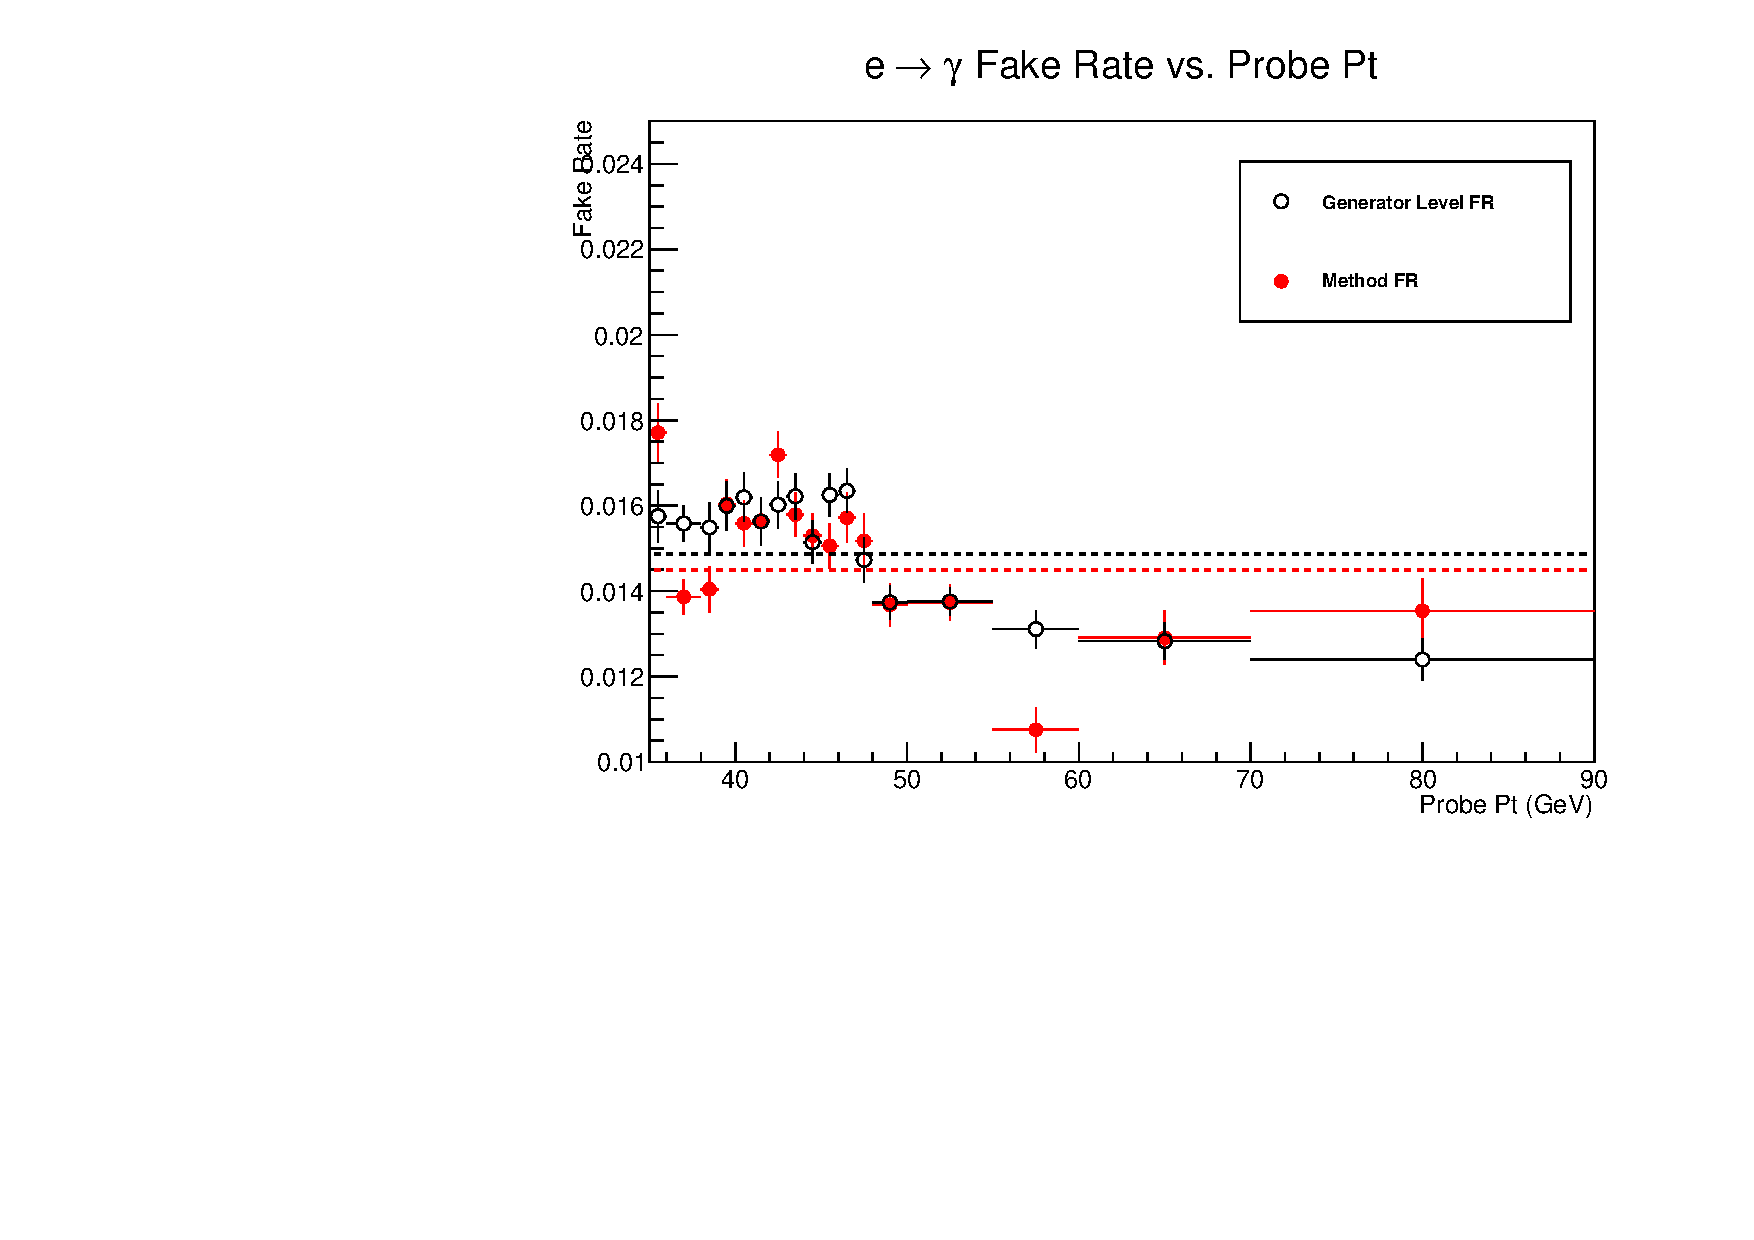
\includegraphics[width=0.45\textwidth]{efake_figs/closure_pt.pdf}}
{\label{closure_pu}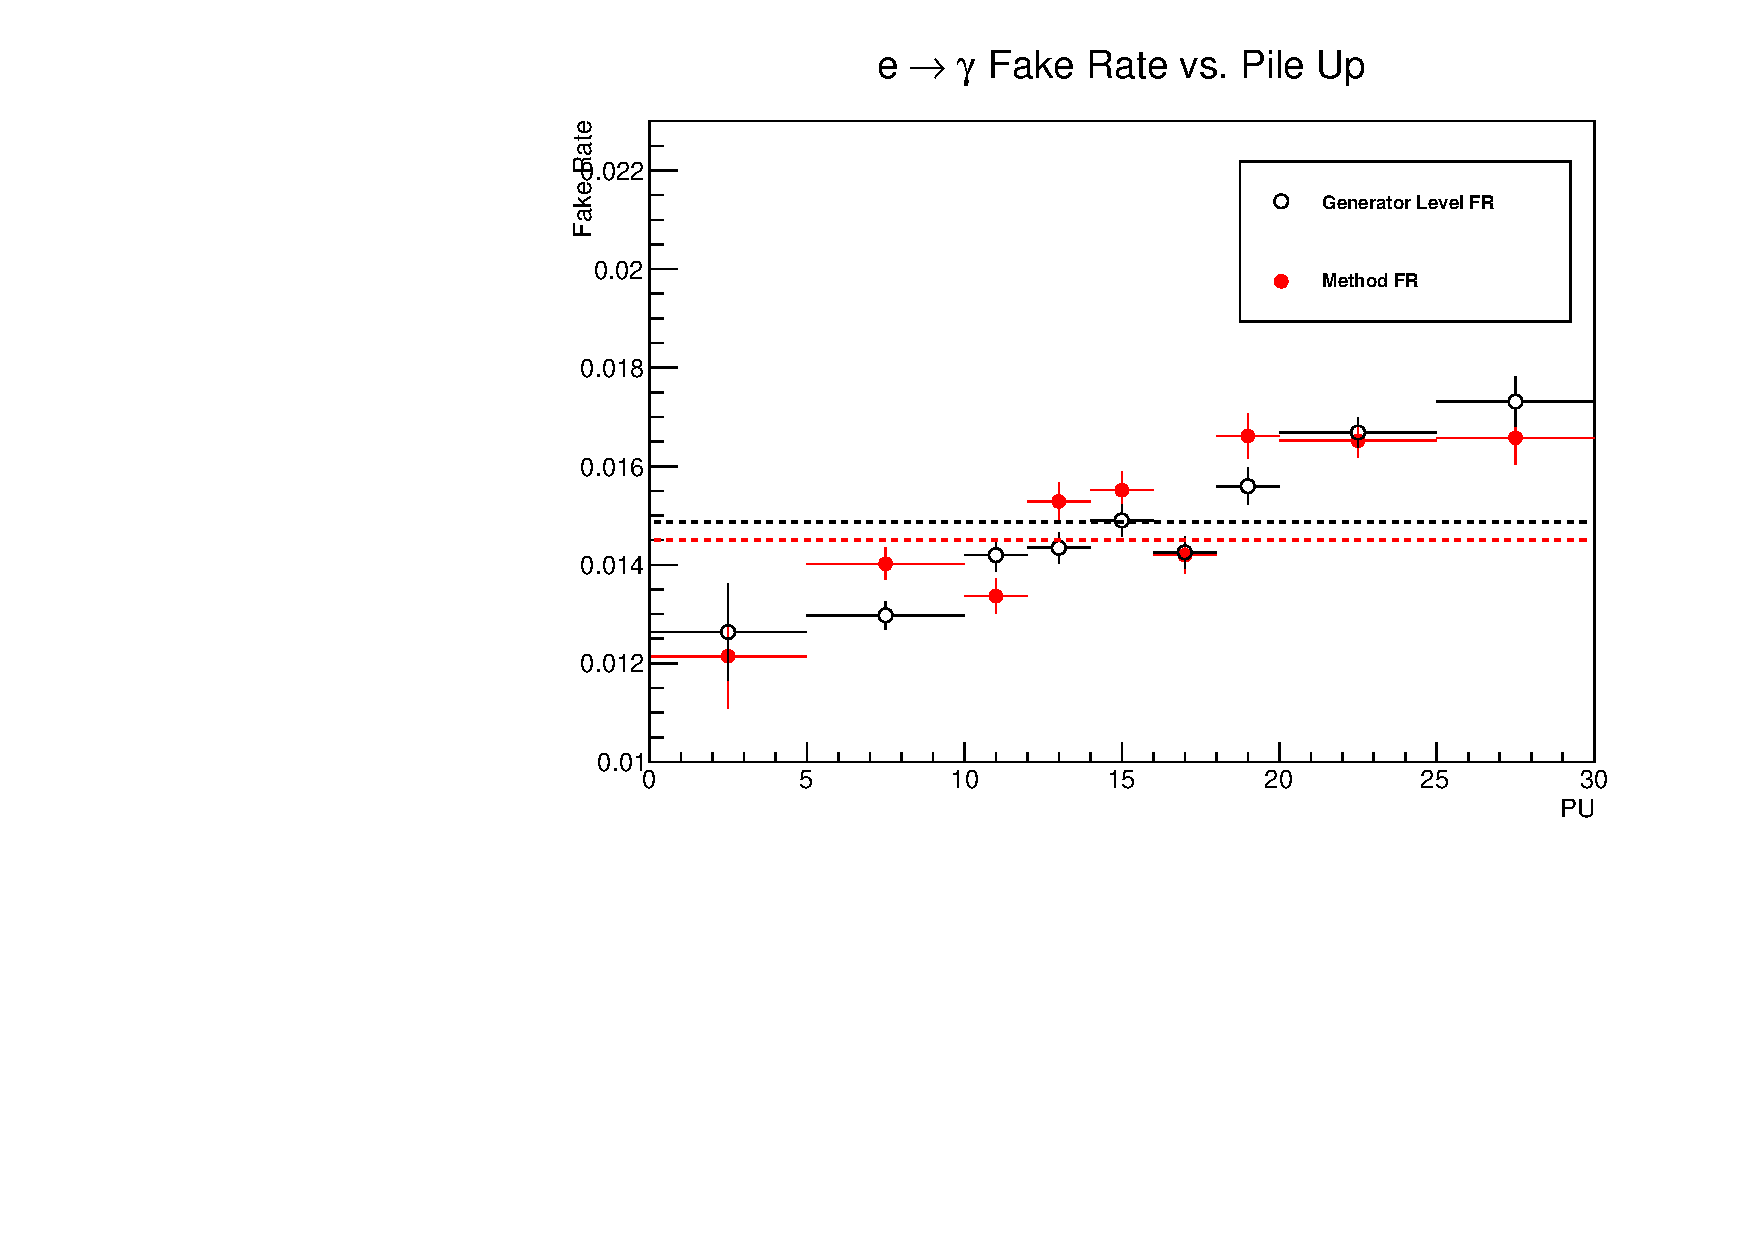
\includegraphics[width=0.45\textwidth]{efake_figs/closure_pu.pdf}}
\\
{\label{closure_ntrk}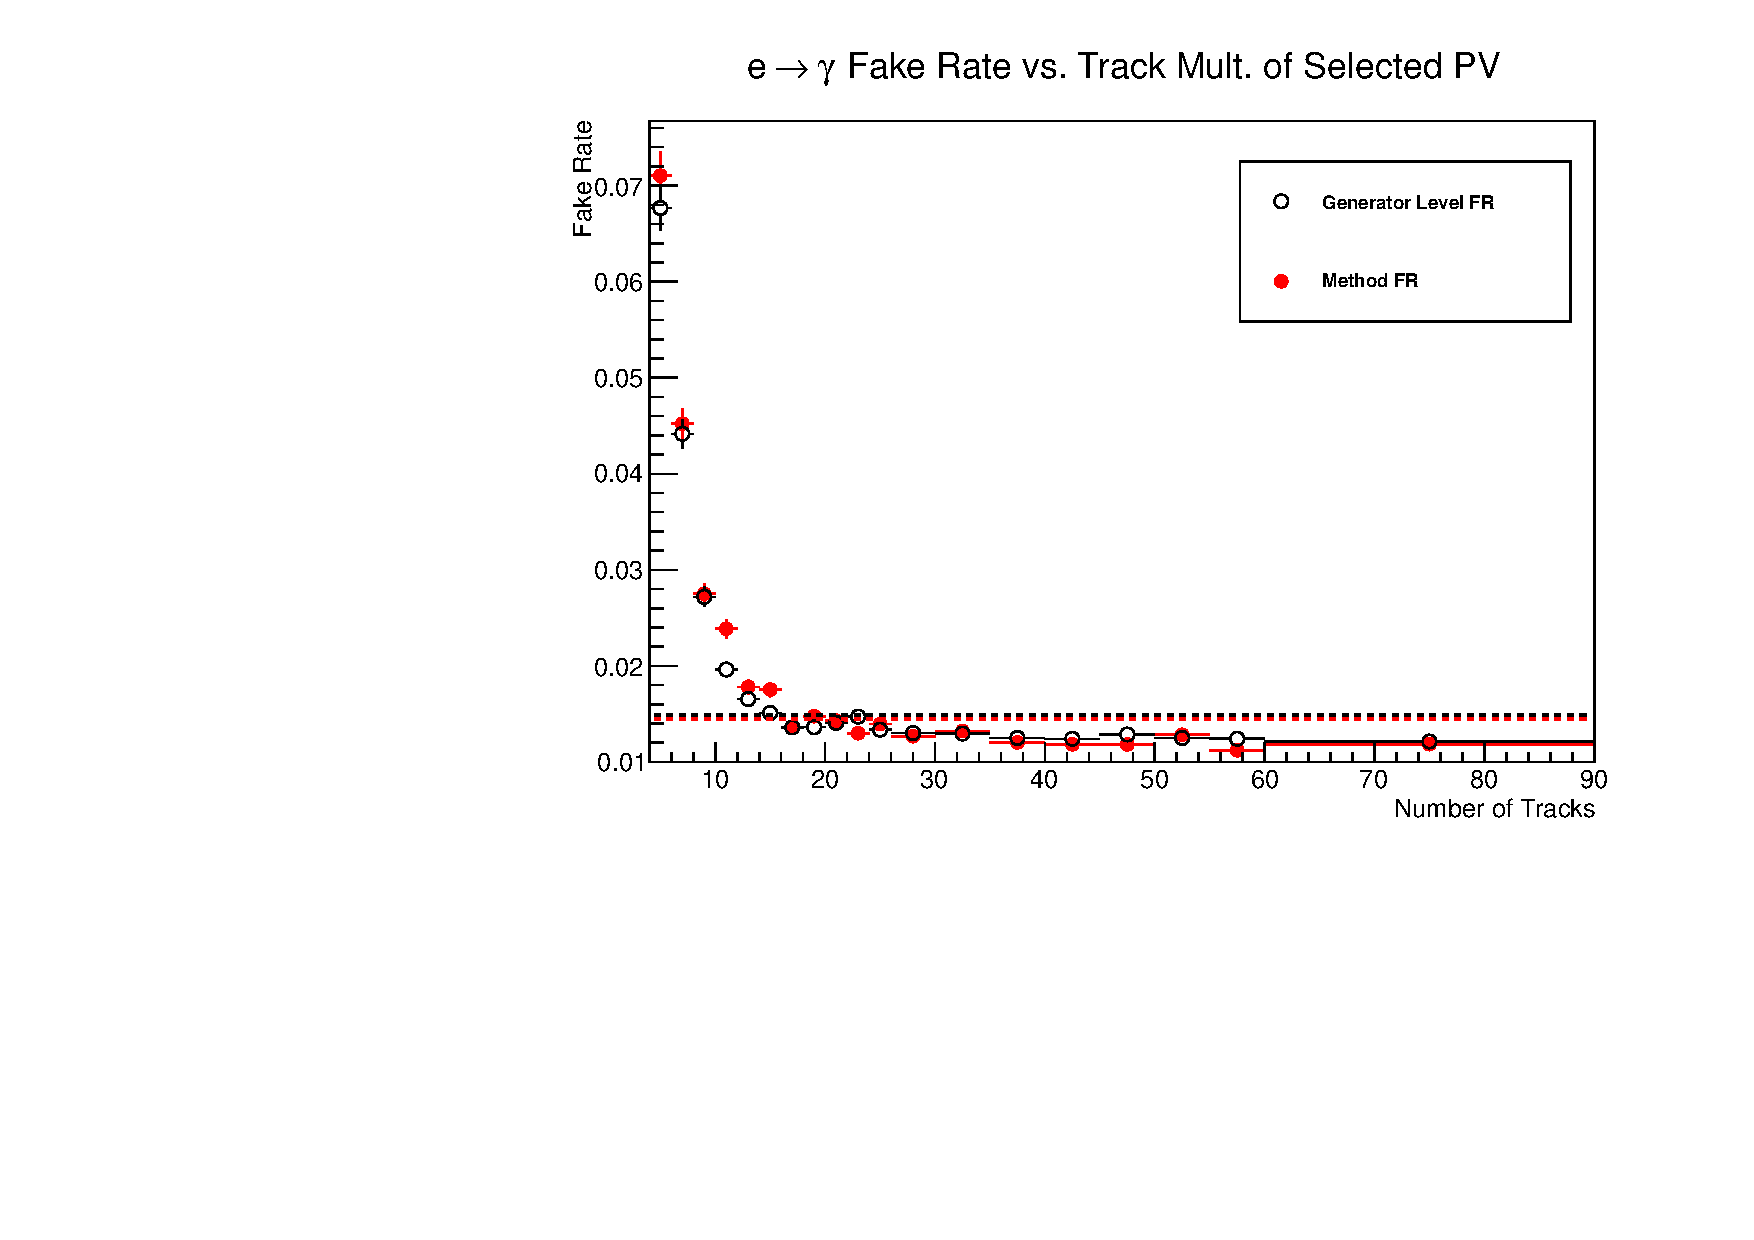
\includegraphics[width=0.45\textwidth]{efake_figs/closure_trk.pdf}}
\caption{PV matched closure test in probe $p_T$,number of reconstructeed primary vertices and track multiplicity}
\label{closure_all}
\end{center}
\end{figure}

%\begin{figure}[H]
%\begin{center}
%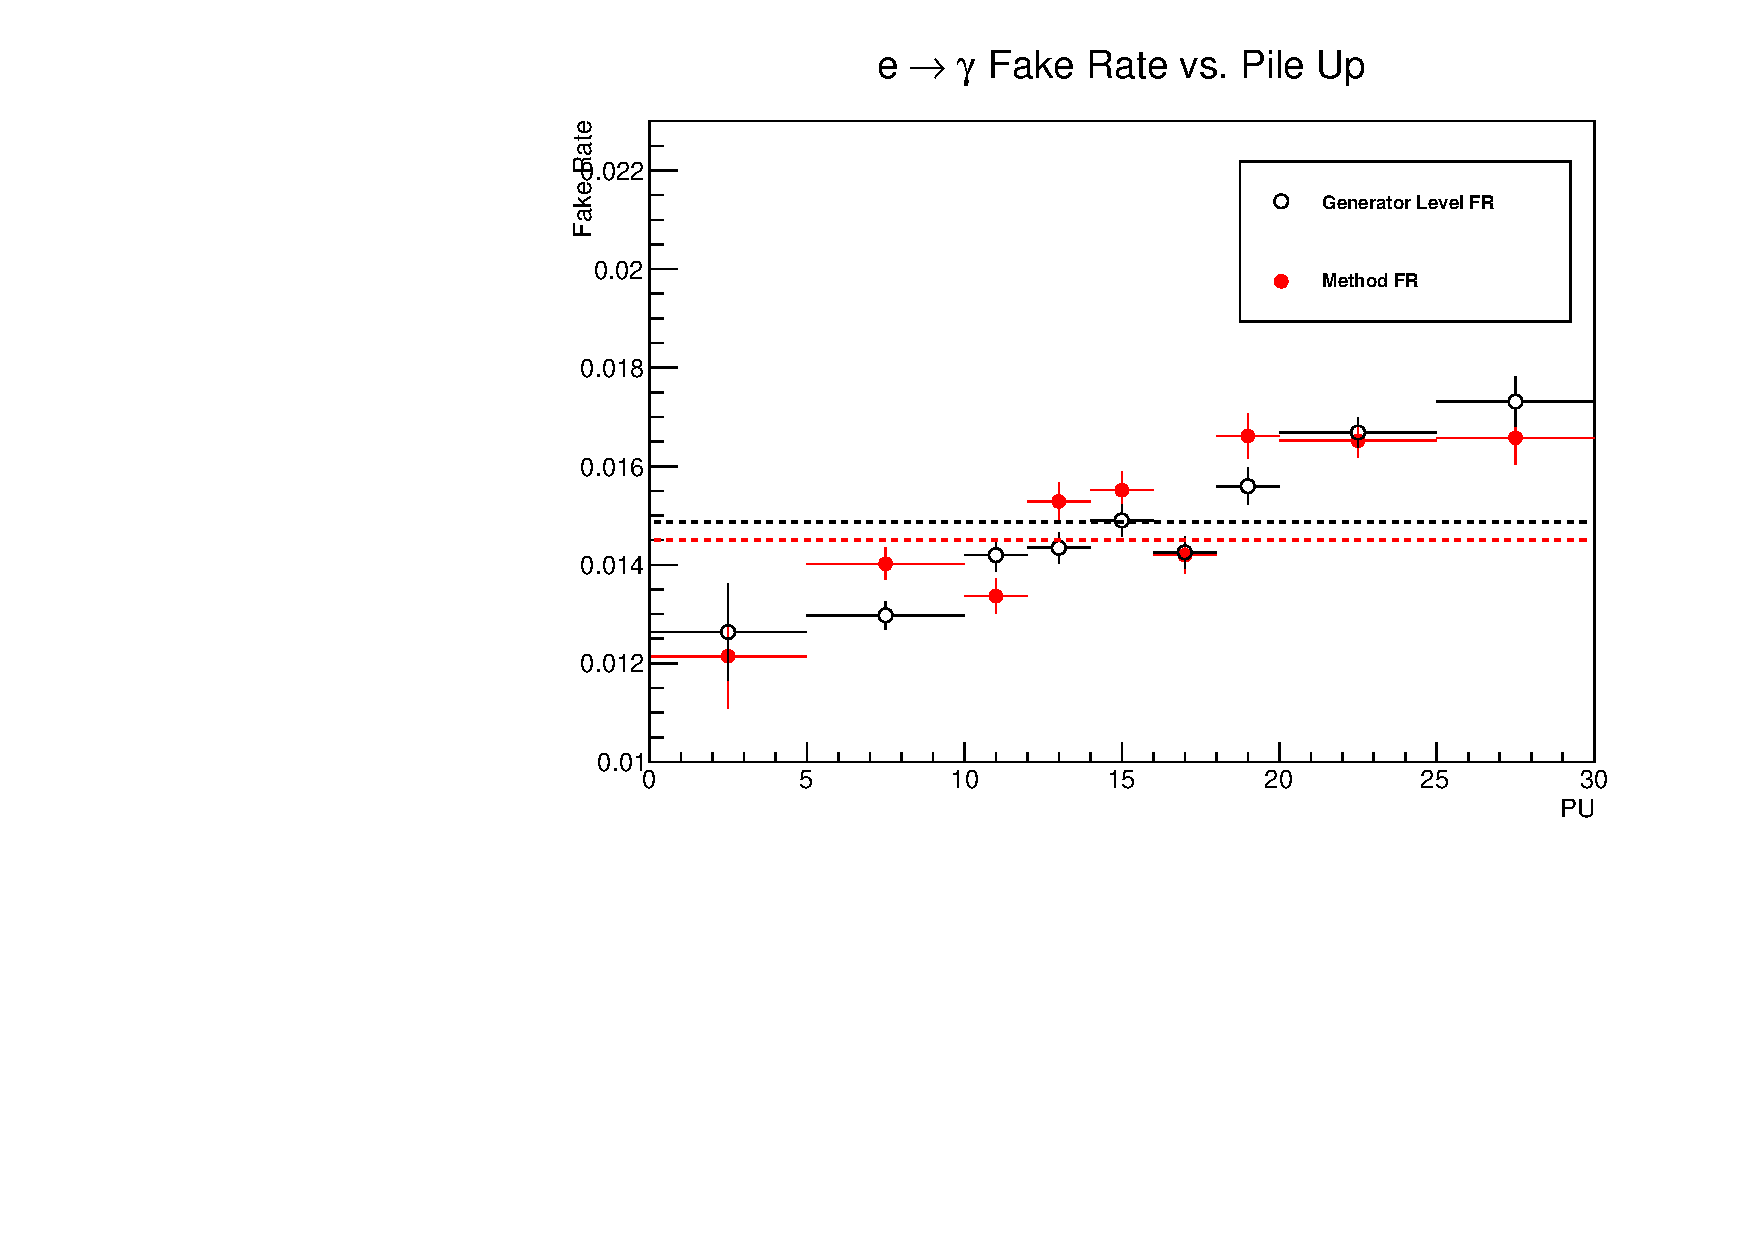
\includegraphics[scale=0.5]{efake_figs/closure_pu.pdf}
%\caption{PV matched closure test in number of reconstructeed primary vertices.}
%\label{closure_pu}
%\end{center}
%\end{figure}

%\begin{figure}[H]
%\begin{center}
%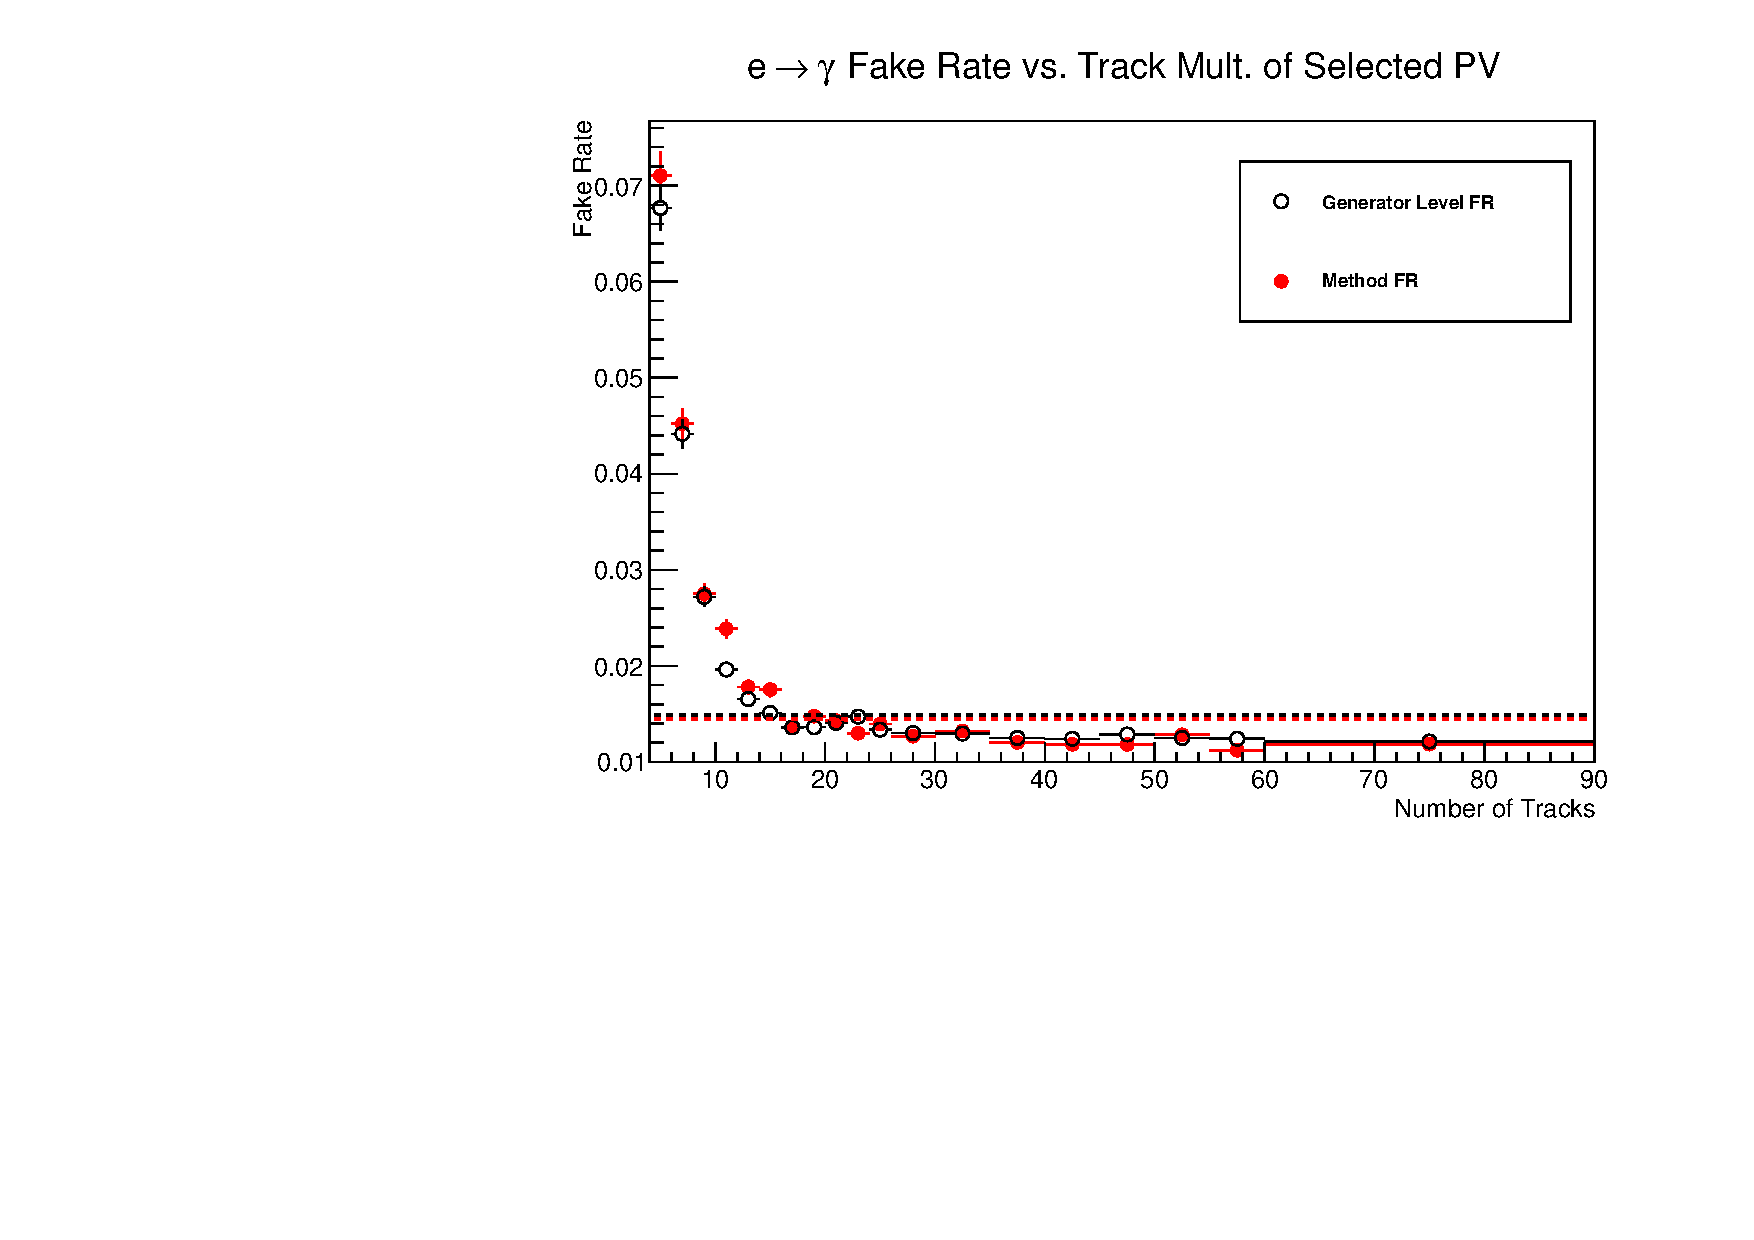
\includegraphics[scale=0.5]{efake_figs/closure_trk.pdf}
%\caption{PV matched closure test in track multiplicity.}
%\label{closure_ntrk}
%\end{center}
%\end{figure}

We can see that the agreement between the gen-level and reco-level fake rates improves and the method closes within 4\%.

\subsubsection{Systematic Uncertainty on the Electron $\rightarrow$ Photon Fake Rate Measurement}
Two of the main systematic errors have been discussed in the previous section:

\begin{itemize}
\item The flat assumption systematic error is found to be 5\% on the number of events;
\item The closure test systematic is found to be 4\% on the value of the fake rate.
\end{itemize}

The remaining systematic uncertainty is related to the background estimation Fig.~\ref{Zeall}, i.e. the choice of the functional form to represent the backgroun composition. Two choices were made for that estimation: a simple decaying exponential and the RooCMSShape. Looking at the full mass spectrum of the invariant mass, without parametrization, the amount of expected background is much smaller than the number of signal events. Because of that, we don't expect the fake rate to be very dependent on the functional shape of the background. Indeed, the difference in the calculated fake rate for the two functions is about 4\%.

These systematic errors are assumed independent and should be added as such in the final number for the fake rate. They are, however, very small compared to the other sources of systematic errors in the analysis.

%  Events with single electrons misidentified as photons are another major source of background.
%  An electron can be misidentified as a photon if the pixel seed in the tracker from the electron's trajectory does not get reconstructed.
%  This background is estimated using a tag-and-probe method with $\Z\to ee$ events. The pixel seed efficiency ($\epsilon_{\gamma_{e}}$) to identify electrons is estimated in the $Z$ boson mass window of 60-120\GeV. The inefficiency ($1-\epsilon_{\gamma_{e}}$) of the pixel seed requirement is found to be $2.31\pm 0.03 \%$. The ratio $(1-\epsilon_{\gamma_{e}})/\epsilon_{\gamma_{e}}$, which represents the electron misidentification rate, is applied to a candidate sample with the inverted pixel seed requirement and used to estimate the contamination in the signal region. The misidentification rate is found to be dependent on the number of vertices reconstructed in the event and the number of tracks associated to the selected primary vertex.   The difference in the final yields using the two parameterizations or the inclusive measurement of $\epsilon_{\gamma_{e}}$ are found to be within $5\%$. This difference is considered as a systematic uncertainty, and the yield calculated using the inclusive rate is used as the nominal estimate. The method is repeated on simulation, and the difference of $4\%$ between the measured and known electron misidentification rate is considered as an additional source of systematic uncertainty.


%The rate of misidentified electrons with respect to these quantities are shown in Figure~\ref{fig:eg_fakerate1}.

%Figures 29.b and c, if necessary
%\begin{figure}[H]
%\centering
%[]{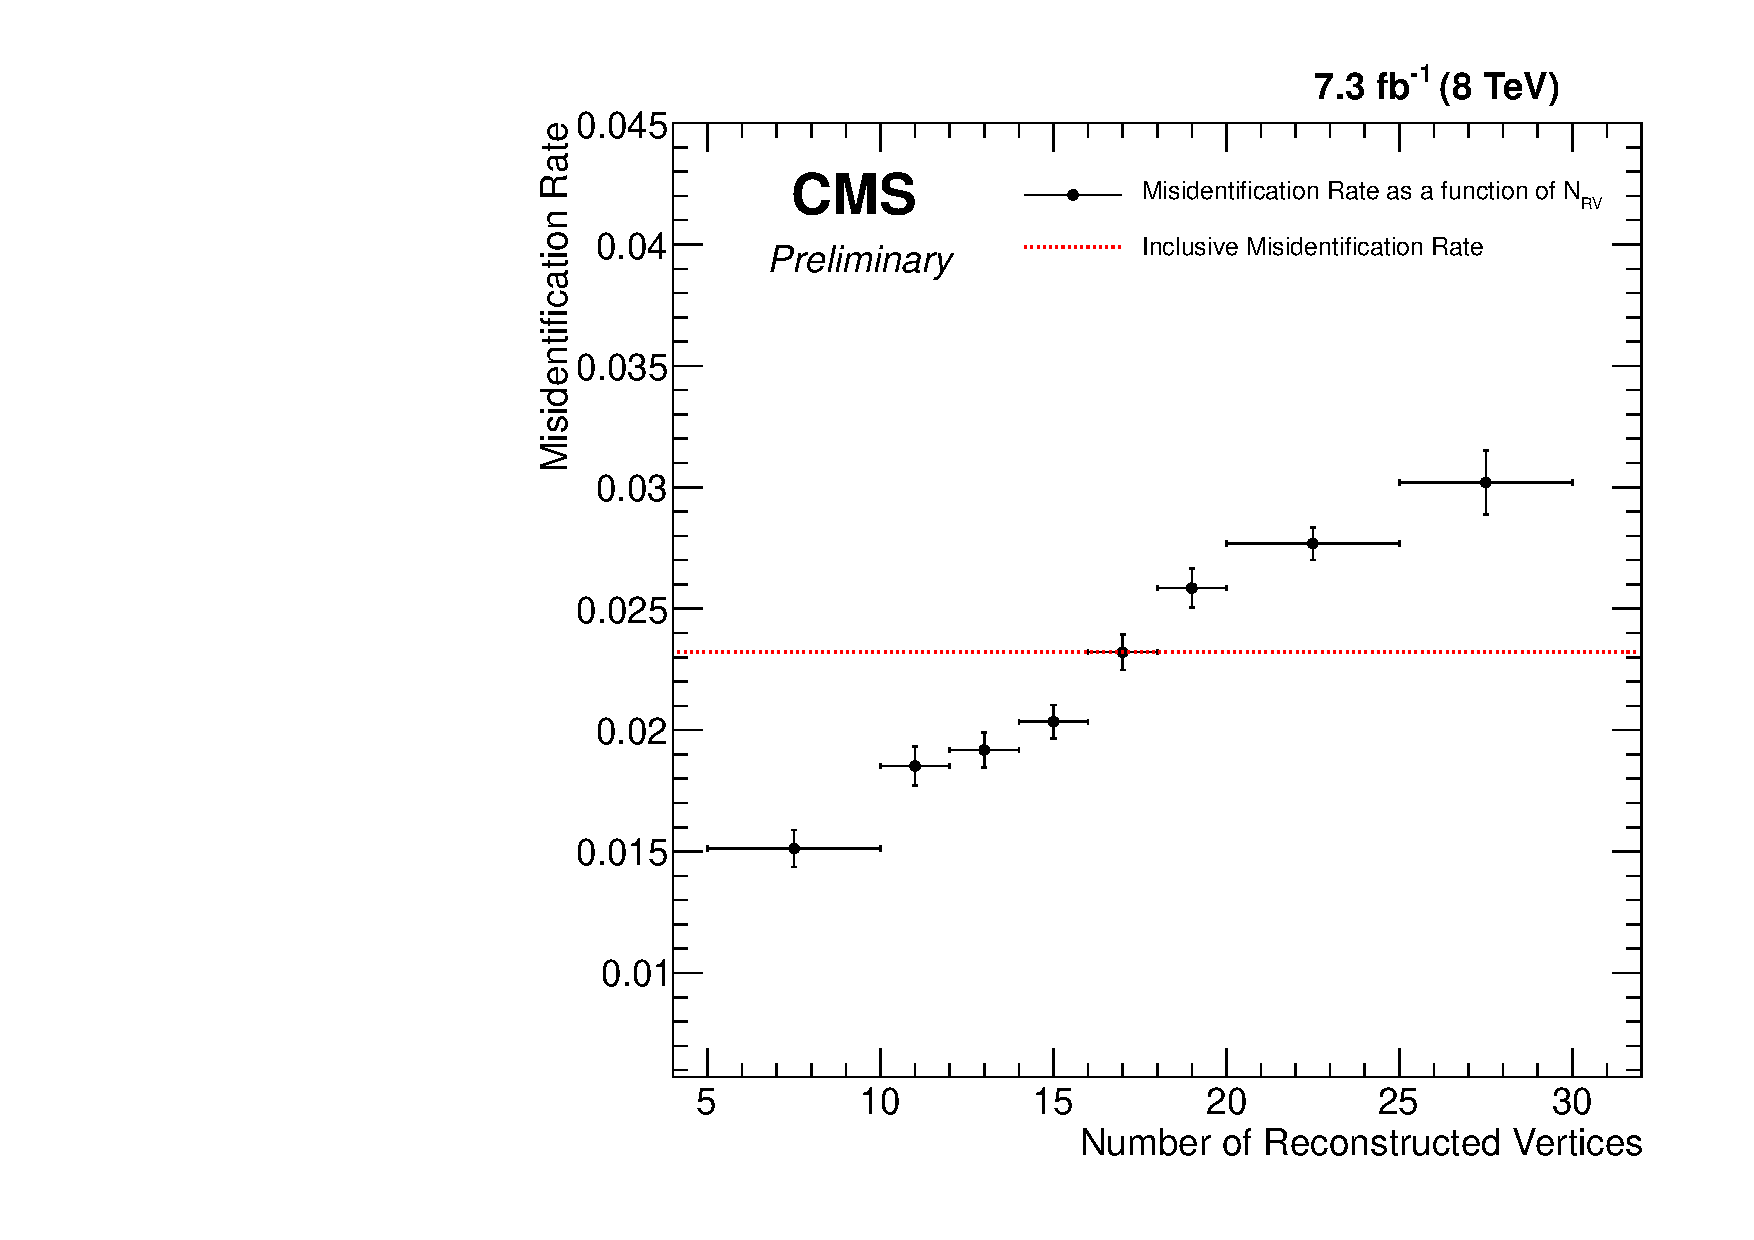
\includegraphics[scale=0.42]{figures/eg_nvtx.pdf}}
%[]{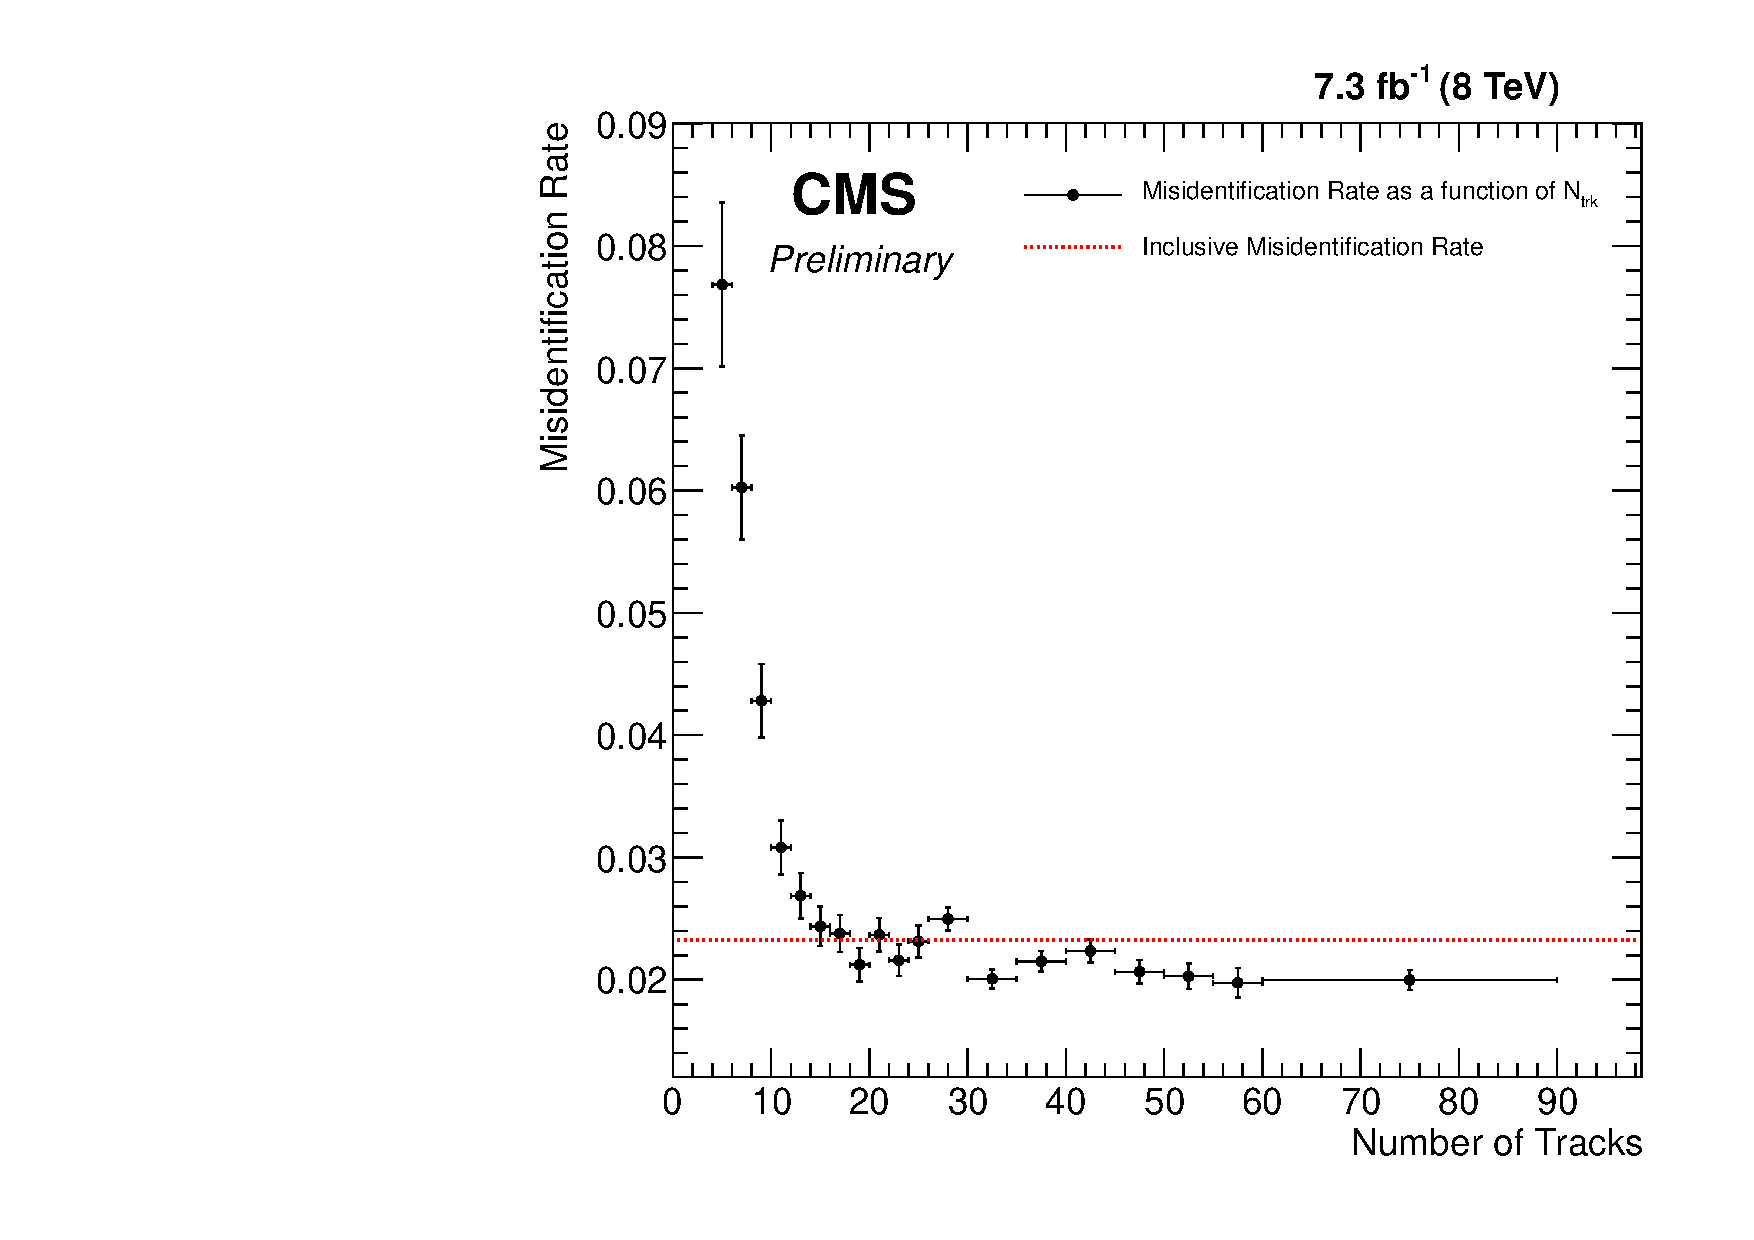
\includegraphics[scale=0.42]{figures/eg_ntrk.pdf}}
%\caption{Rate of electrons misidentified as photons ($1-\epsilon_{\gamma_{e}}$) parametrized as a function of the number of reconstructed vertices (a) and number of tracks associated to the primary vertex (b). The red line represents the inclusive measurement of $\epsilon_{\gamma_{e}}$.}
%\label{fig:eg_fakerate1}
%\end{figure}


\subsection{Non-collision background estimates from data}

The search is susceptible to contamination from non-collision backgrounds which arise from cosmic ray interactions, spurious signals in the ECAL, and accelerator induced secondary particles (beam halo). These backgrounds have different arrival time distributions compared to prompt photons produced in hard scattering. To quantify the contamination due to these backgrounds a fit is performed to the candidate time distribution using background templates derived from the data. The contamination due to out-of-time background contribution is found to be negligible, therefore not included in the final event yield.

\subsection{Background modeling validation}

The background modeling is examined in several control regions. A control sample enriched in $W(l\nu)\gamma$ events is defined with inverted lepton-veto requirement in the preselection, thus selecting events with a loose $e$ or $\mu$. It is expected to be free of any signal contamination due to the presence of a lepton. Another control sample enriched in $\gamma +$jet events is constructed by just requiring no selection other than the preselection requirements. Figure~\ref{fig:CR12} shows the data vs SM expectation in the two control regions. The observed data and estimated SM backgrounds are found to be consistent both in yield and shape.

 %% figure for control regions 
\begin{figure}[H]                  
\centering   
[]{\label{fig:QCDPt}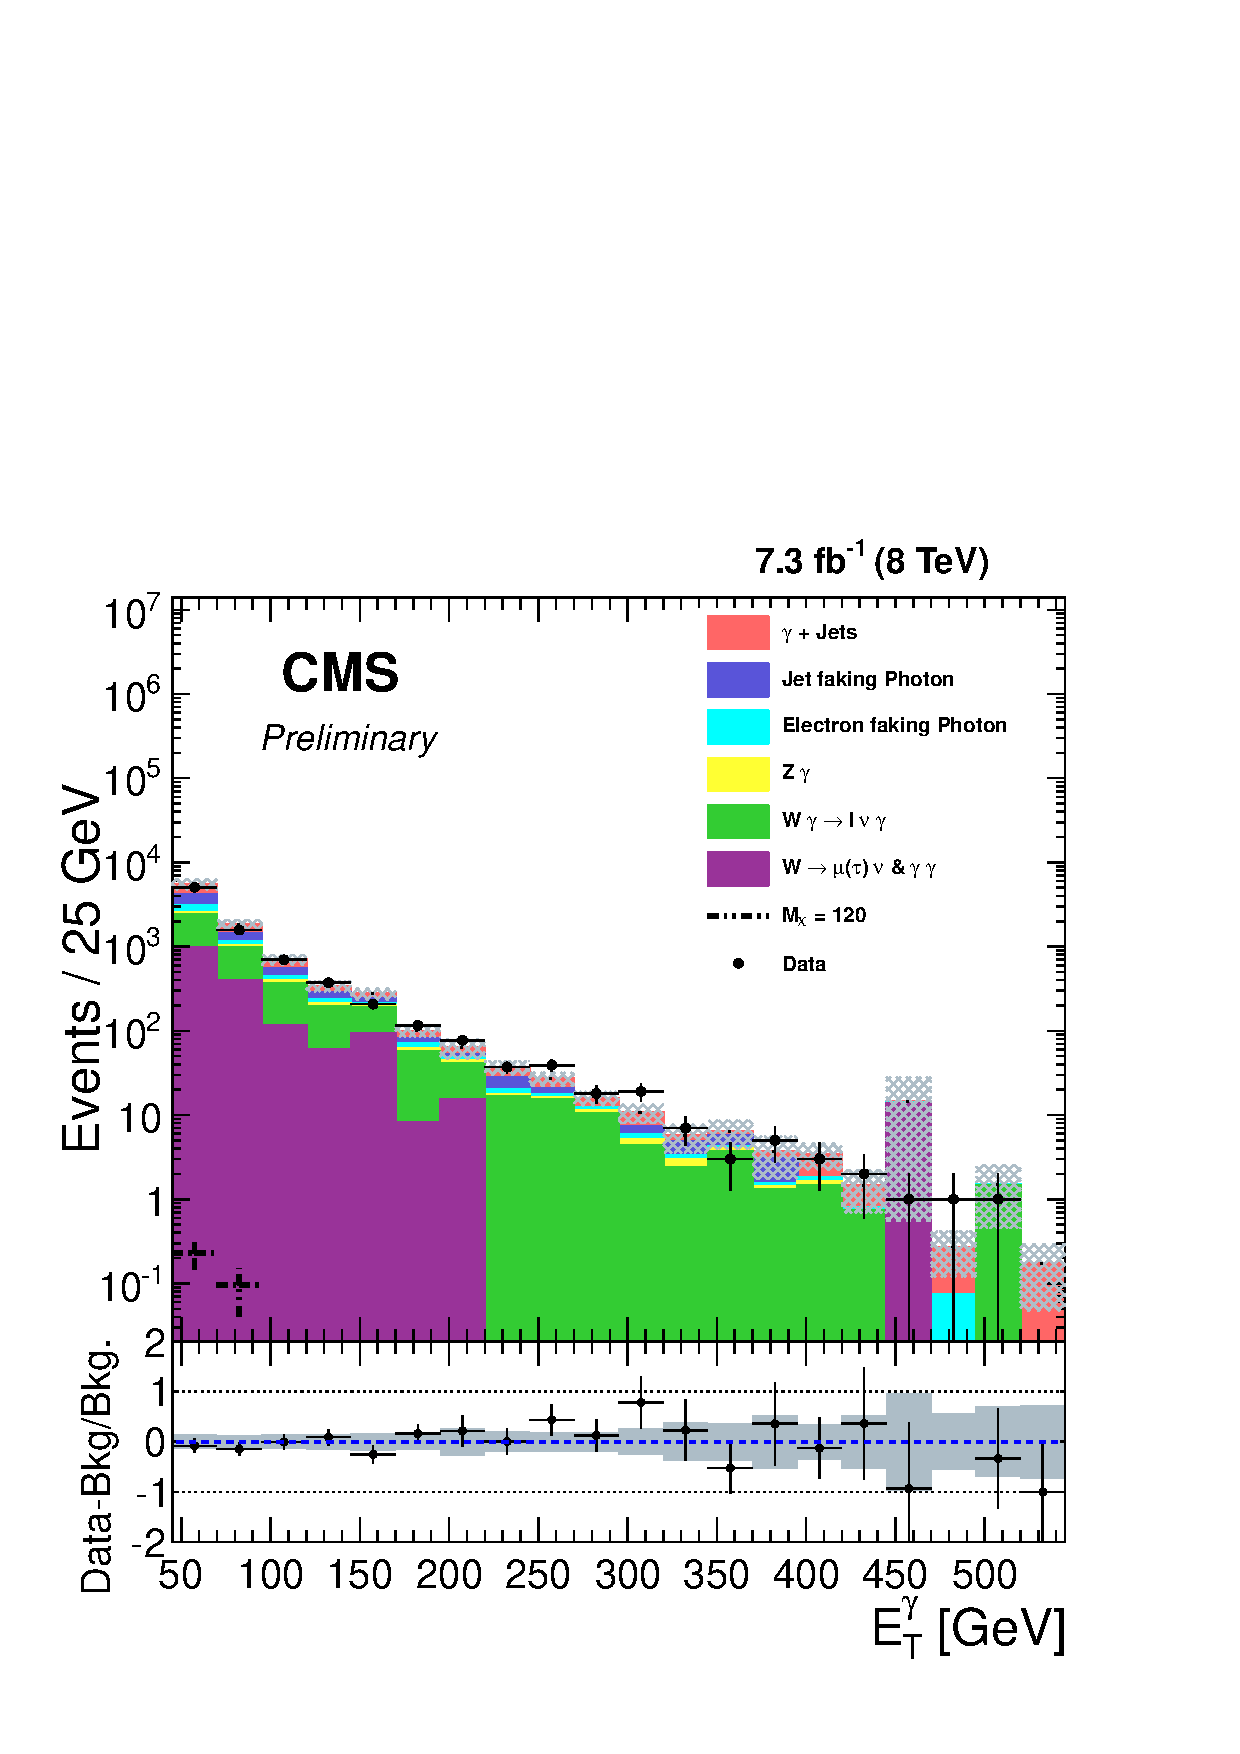
\includegraphics[width=0.45\textwidth]{PAS_Plots2/StackedHisto_Pho_Pt_LeptonCR.pdf}}
[]{\label{fig:QCDMET}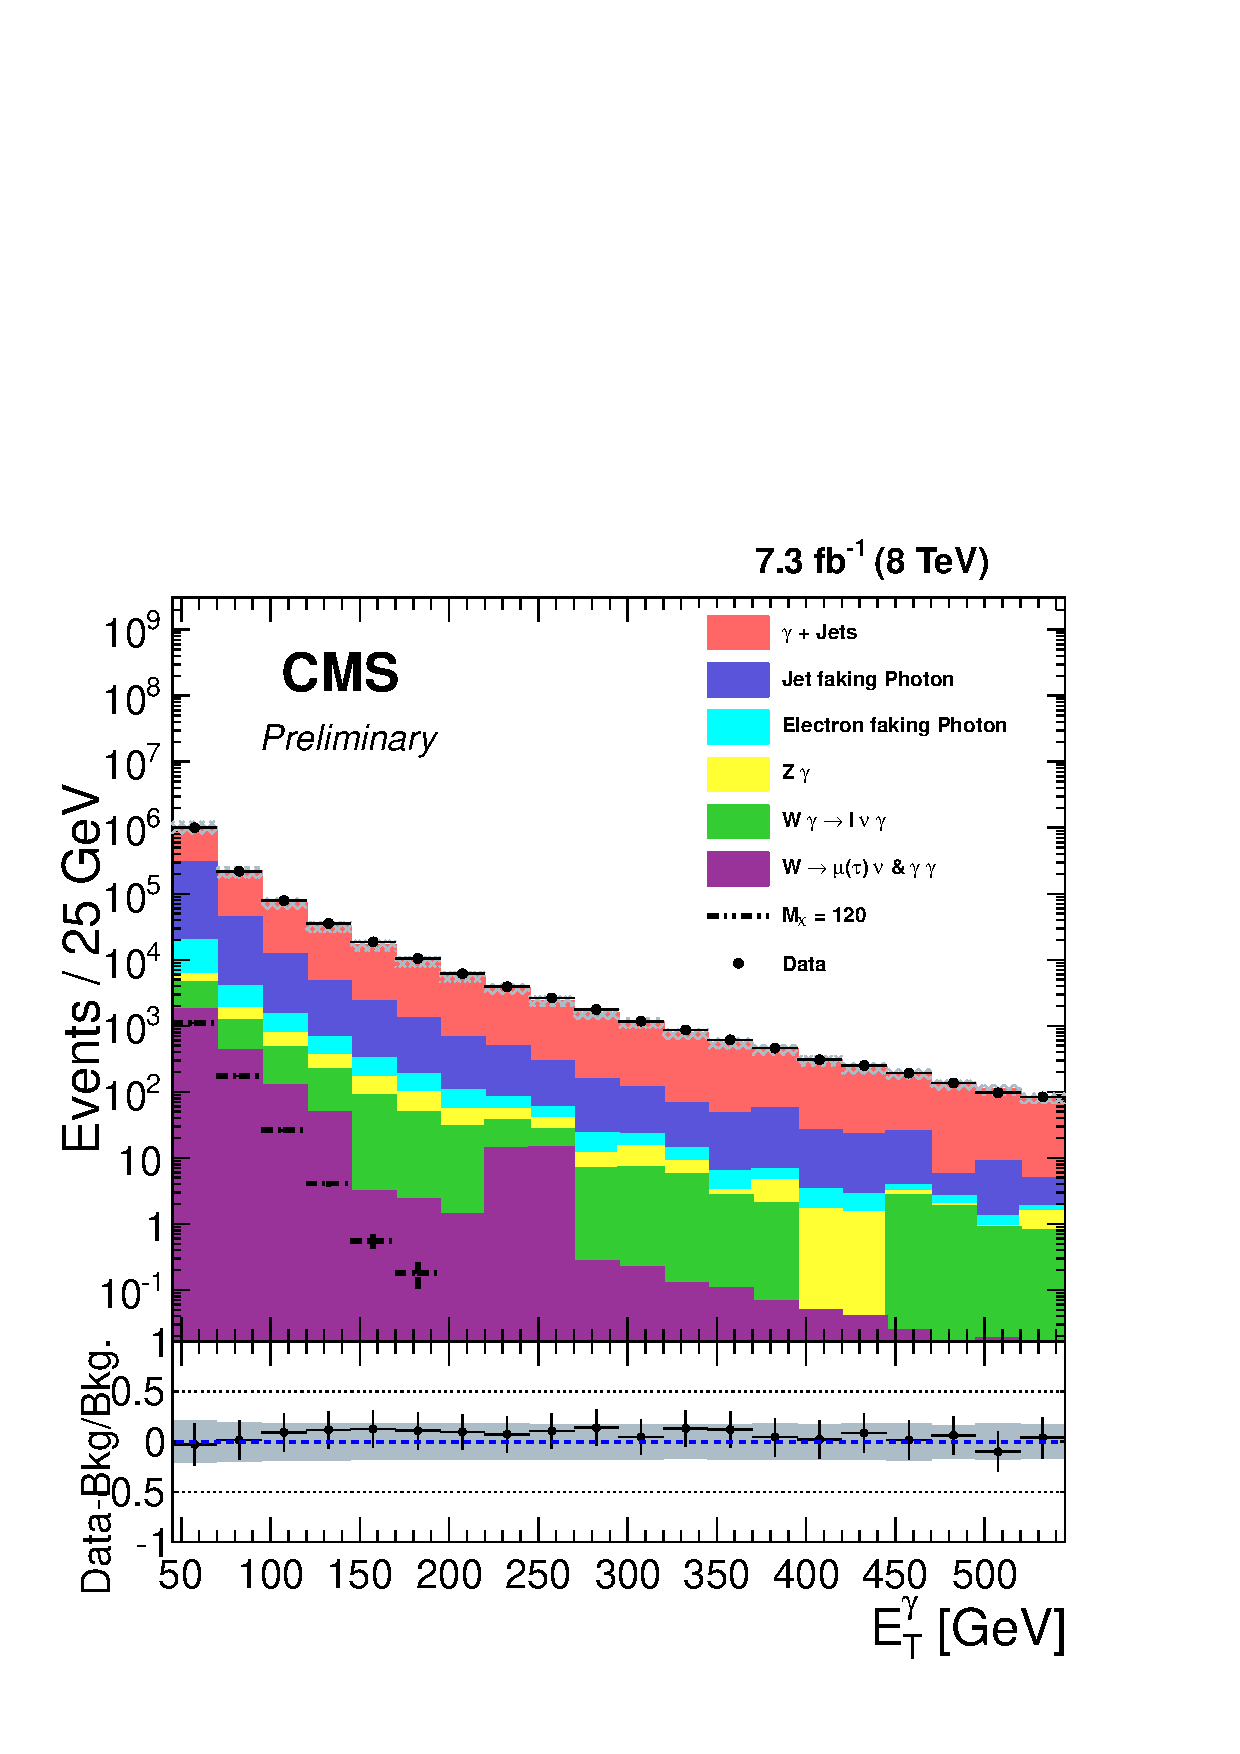
\includegraphics[width=0.45\textwidth]{PAS_Plots2/StackedHisto_Pho_Pt_Preliminary.pdf}}
%[]{\label{fig:QCDPt}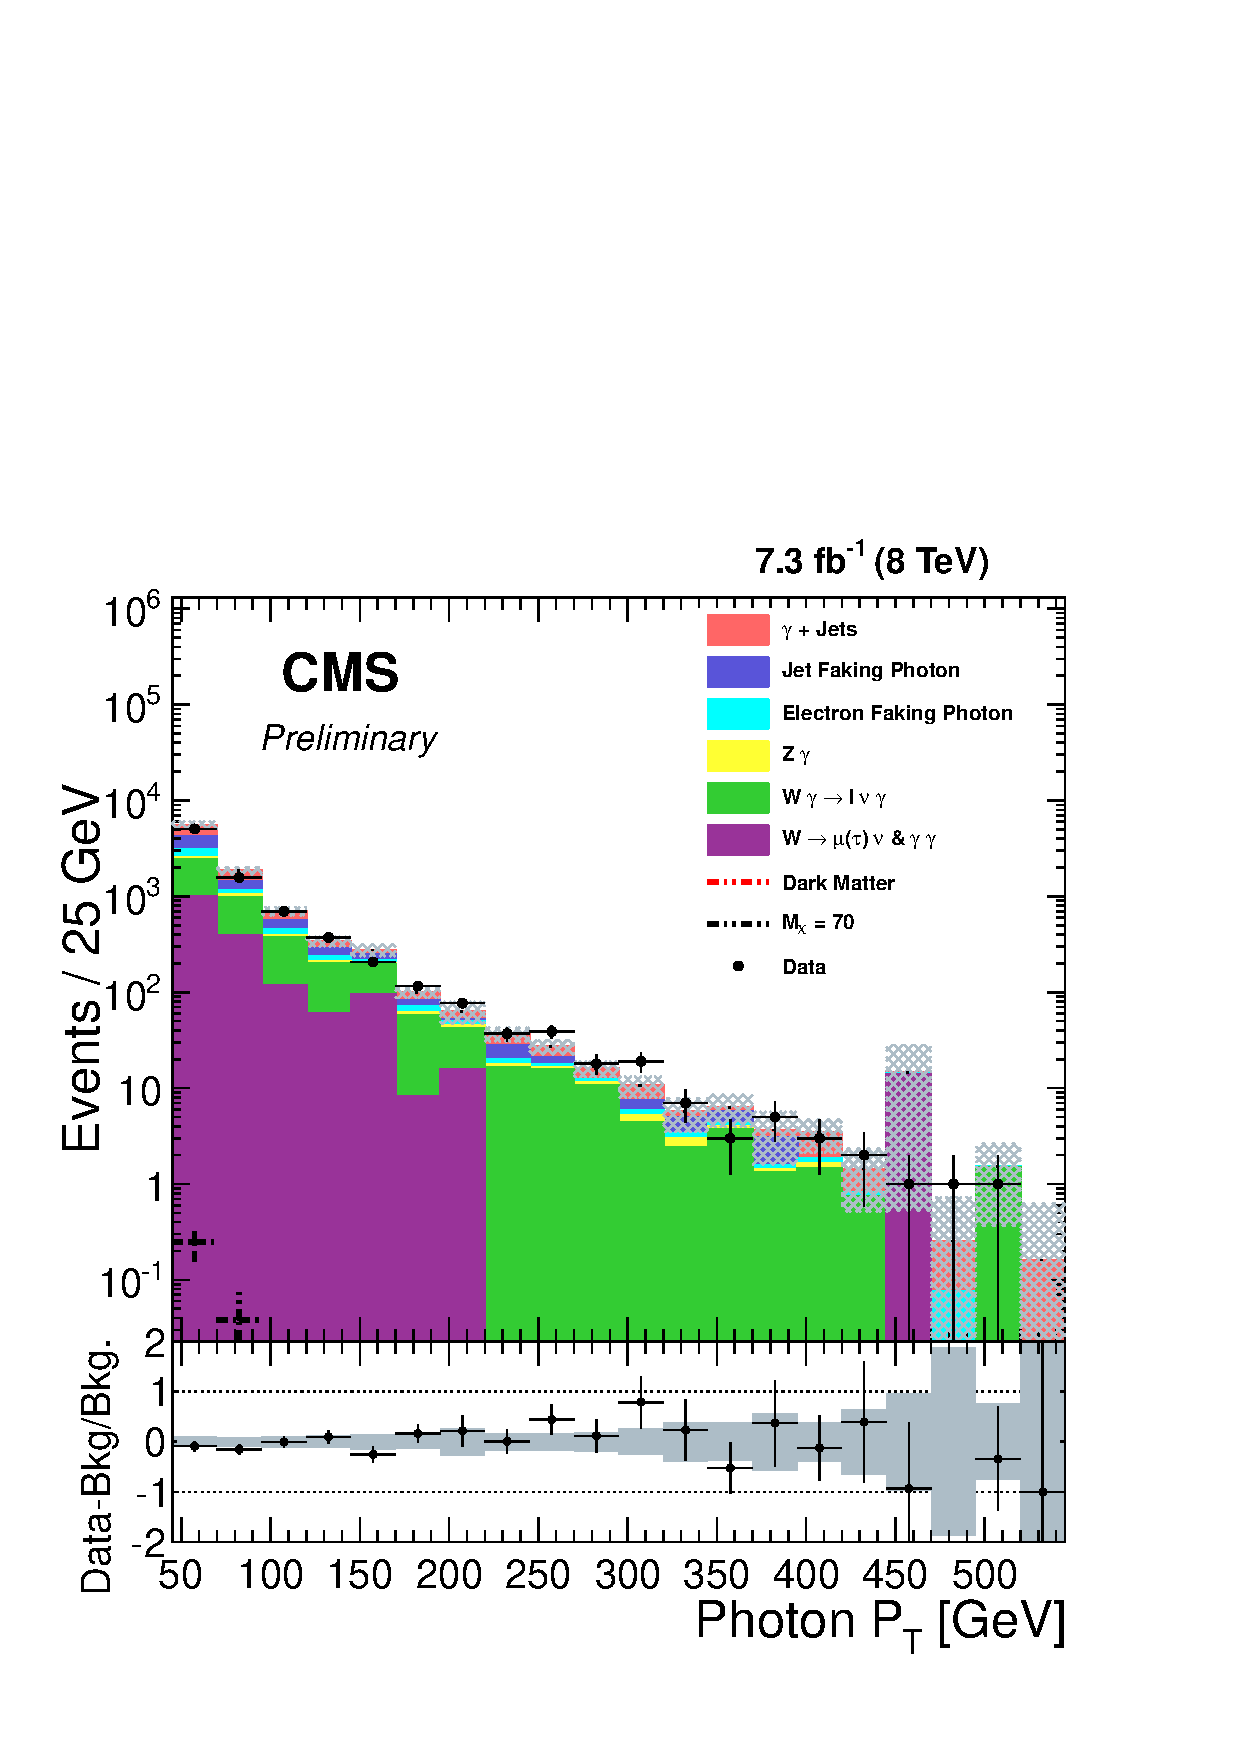
\includegraphics[scale=0.4]{figures/lepton_pt_CR.pdf}}                           
%[]{\label{fig:QCDMET}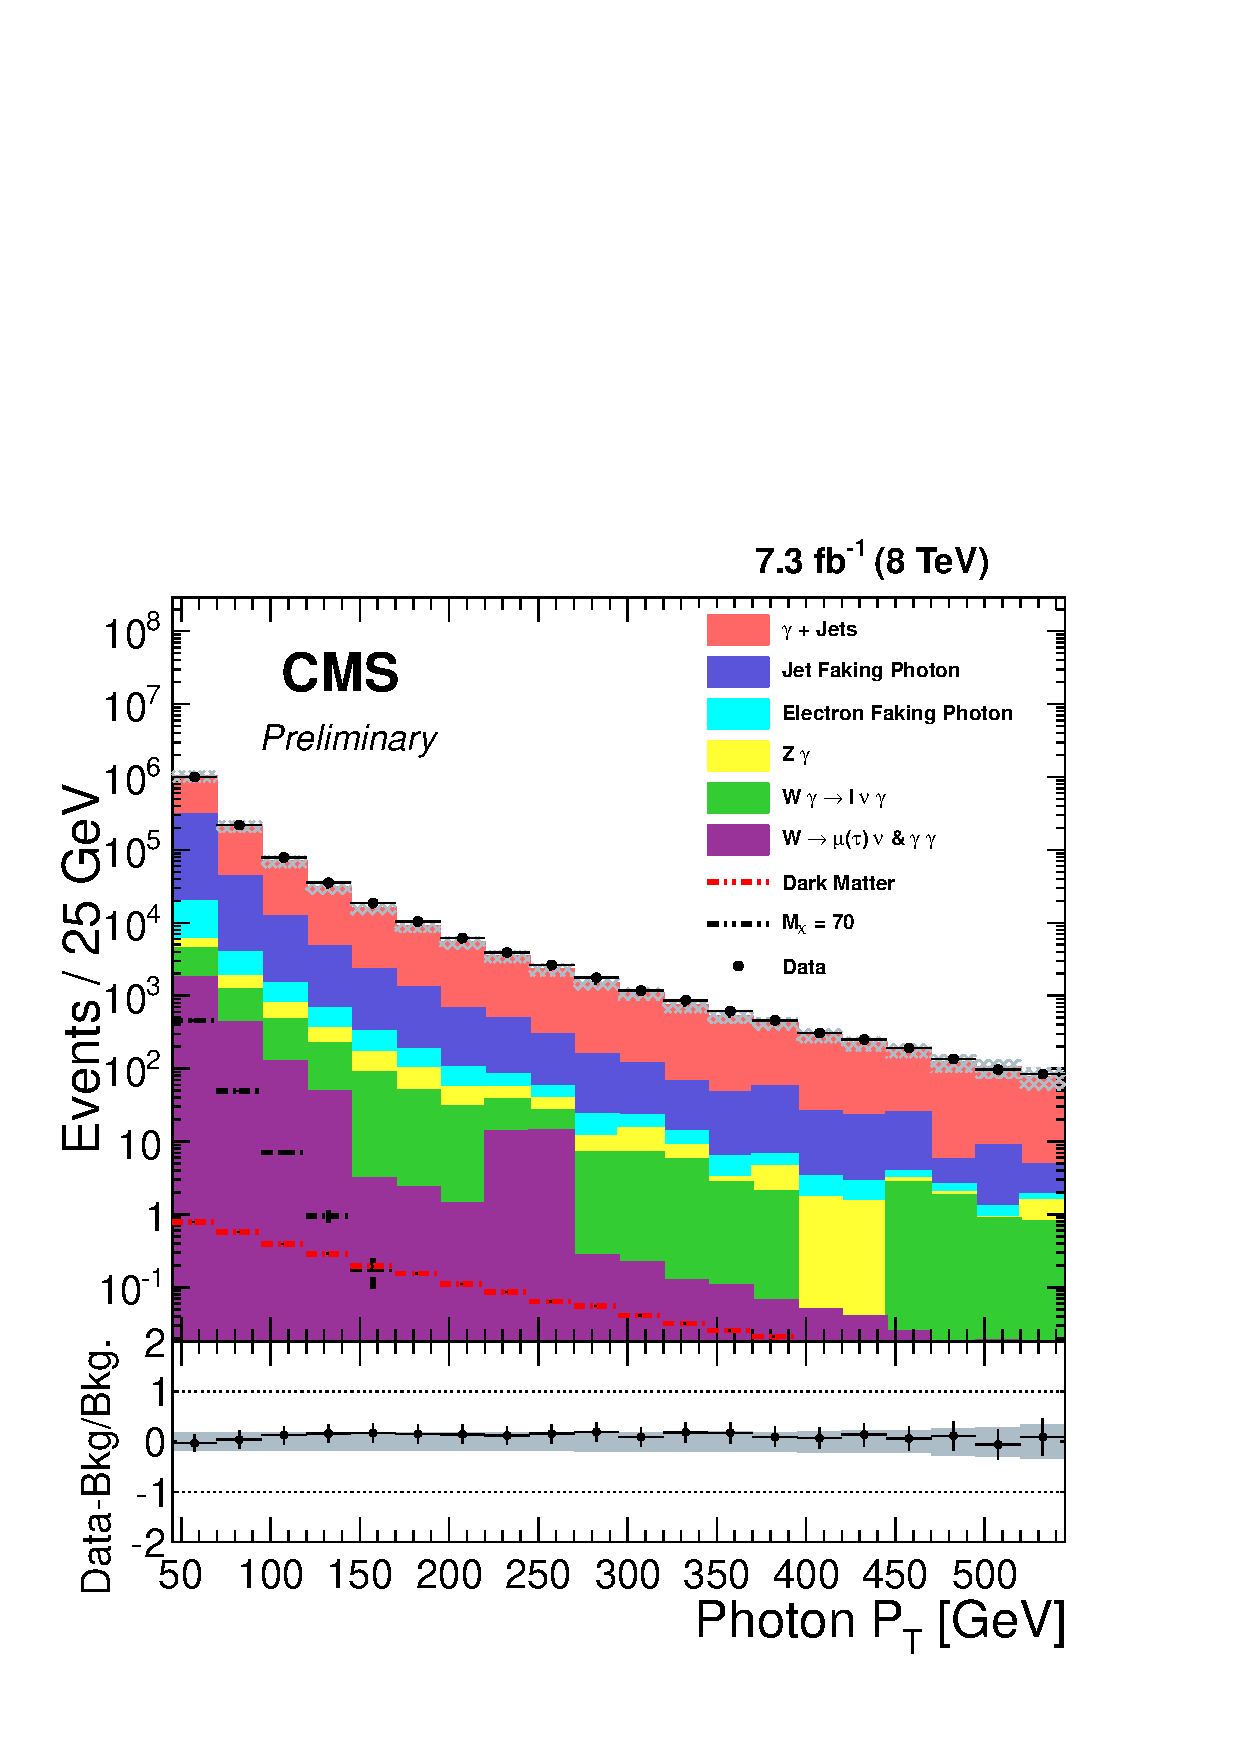
\includegraphics[scale=0.4]{figures/QCD_pt_CR.pdf}}                         
\caption{The \etg distributions for data vs. SM expectation in a control region enriched by (a)  W($l\nu$) events, and (b) $\gamma+$jet events. The bottom panels in each plot show the ratio of (data - background)/background and the gray band includes both the statistical and systematic uncertainty on the background prediction.}
\label{fig:CR12}                     
\end{figure} 

  
